
\documentclass[letterpaper,12pt,titlepage,oneside,final]{book}
 

\newcommand{\package}[1]{\textbf{#1}} 
\newcommand{\cmmd}[1]{\textbackslash\texttt{#1}} 
\newcommand{\href}[1]{#1} 

\usepackage{algorithm}
\usepackage[noend]{algpseudocode}
\usepackage{algorithmicx}

\algnewcommand\algorithmicInput{\textbf{Input:}}
\algnewcommand\Input{\item[\algorithmicInput]}

\algnewcommand\algorithmicOutput{\textbf{Output:}}
\algnewcommand\Output{\item[\algorithmicOutput]}

\newcommand\abs[1]{\left|#1\right|}

\algdef{SE}[DOWHILE]{Do}{doWhile}{\algorithmicdo}[1]{\algorithmicwhile\ #1}


\usepackage{ifthen}
\usepackage{indentfirst}
\newboolean{PrintVersion}
\setboolean{PrintVersion}{false} 

\usepackage{amsmath,amssymb,amstext,amsthm}
\usepackage[pdftex]{graphicx}

\newcommand\Tstrut{\rule{0pt}{2.6ex}}
\newcommand\Bstrut{\rule[-0.9ex]{0pt}{0pt}}
\newcommand{\TBstrut}{\Tstrut\Bstrut}

\usepackage{lipsum}
\newcounter{examplecounter}
\newenvironment{example}{\begin{quote}%
    \refstepcounter{examplecounter}%
  \textbf{Example \arabic{examplecounter}}%
  \quad
}{%
\end{quote}%
}

\newcounter{definitioncounter}
\newenvironment{defn}{\begin{quote}%
    \refstepcounter{definitioncounter}%
  \textbf{Definition \arabic{definitioncounter}}%
  \quad
}{%
\end{quote}%
}

\newcounter{notecounter}
\newenvironment{note}{\begin{quote}%
    \refstepcounter{notecounter}%
  \textbf{Note \arabic{notecounter}}%
  \quad
}{%
\end{quote}%
}

\newcounter{theoremcounter}
\newenvironment{theorem}{\begin{quote}%
    \refstepcounter{theoremcounter}%
  \textbf{Theorem \arabic{theoremcounter}}%
  \quad
}{%
\end{quote}%
}

\newcounter{Table}
\usepackage{scrextend}

\usepackage{multirow}

\usepackage[pdftex,letterpaper=true,pagebackref=false]{hyperref} 

\usepackage[toc,page]{appendix}
    
\hypersetup{
    plainpages=false,       % needed if Roman numbers in frontpages
    pdfpagelabels=true,     % adds page number as label in Acrobat's page count
    bookmarks=true,         % show bookmarks bar?
    unicode=false,          % non-Latin characters in Acrobat’s bookmarks
    pdftoolbar=true,        % show Acrobat’s toolbar?
    pdfmenubar=true,        % show Acrobat’s menu?
    pdffitwindow=false,     % window fit to page when opened
    pdfstartview={FitH},    % fits the width of the page to the window
    pdftitle={uWaterloo\ LaTeX\ Thesis\ Template},    % title: CHANGE THIS TEXT!
%    pdfauthor={Author},    % author: CHANGE THIS TEXT! and uncomment this line
%    pdfsubject={Subject},  % subject: CHANGE THIS TEXT! and uncomment this line
%    pdfkeywords={keyword1} {key2} {key3}, % list of keywords, and uncomment this line if desired
    pdfnewwindow=true,      % links in new window
    colorlinks=true,        % false: boxed links; true: colored links
    linkcolor=blue,         % color of internal links
    citecolor=green,        % color of links to bibliography
    filecolor=magenta,      % color of file links
    urlcolor=cyan           % color of external links
}
\ifthenelse{\boolean{PrintVersion}}{   
\hypersetup{  % override some previously defined hyperref options
%    colorlinks,%
    citecolor=black,%
    filecolor=black,%
    linkcolor=black,%
    urlcolor=black}
}{} % end of ifthenelse (no else)


\setlength{\marginparwidth}{0pt} 
\setlength{\marginparsep}{0pt}
\setlength{\evensidemargin}{0.125in}
\setlength{\oddsidemargin}{0.125in}
\setlength{\textwidth}{6.375in} 
\raggedbottom


\setlength{\parskip}{\medskipamount}


%\renewcommand{\baselinestretch}{1} 
\usepackage{setspace}
\usepackage{etoolbox}

\let\origdoublepage\cleardoublepage
\newcommand{\clearemptydoublepage}{%
  \clearpage{\pagestyle{empty}\origdoublepage}}
\let\cleardoublepage\clearemptydoublepage

\doublespacing

%======================================================================
%   L O G I C A L    D O C U M E N T -- the content of your thesis
%======================================================================
\begin{document}

\title{Modular Algorithms for Computation of Groebner Bases}
\date{2016-03-29}
\author{Ellen Arteca}

\frontmatter
\maketitle
\tableofcontents
\listoffigures
\mainmatter

%======================================================================
\chapter{Introduction}
%======================================================================

\section{Problem Statement}

The computation of Groebner bases is a classic example of a problem suffering from intermediate expression swell in computer algebra.  Efficient computation of Groebner bases would be useful for a range of applications in algebra, including solutions of systems of equations and computational geometry.  This thesis will implement and examine the comparative efficiency of two modular reconstruction methods, Garner's Algorithm for Chinese Remainder computation, and Hensel's Algorithm for ${p}$-adic reconstruction, when applied to Groebner basis computation working over modular integers to reduce expression swell.  

THIS SHOULD BE IN THE ABSTRACT I THINK
Timings tests were performed over a set of problems representing a range of input ideals.  All computations were done using the Maple computer algebra system and interfacing with its supplied Groebner package.  

%----------------------------------------------------------------------
\section{Brief Overview and History of Groebner Bases}
%----------------------------------------------------------------------
 
The concept of a Groebner basis and an algorithm for its computation was introduced by Bruno Buchberger in his 1965 Ph.D. thesis.  The theory can be described in terms of a generalization of univariate polynomial theory.  Briefly: considering polynomial ring ${F[x]}$, field ${F}$ extended by the indeterminate ${x}$, any ideal ${I \subseteq F[x]}$ is cyclic (i.e. can be generated by a single element), which is the greatest common divisor (GCD) of all the elements of ${I}$.  In other words, given a generating set for ${I}$, ${I = <f_1, \ldots, f_s>}$ for ${\{f_1, \ldots, f_s\} \subseteq F[x]}$, the GCD ${d = \gcd(f_1, \ldots, f_r)}$ can be computed so that ${I}$ can be written equivalently as ${I = <d>}$.  Then, for any polynomial ${f \in F[x]}$, membership in the ideal ${I}$ is satisfied ${\iff}$ ${d | f}$ i.e. ${f}$ is also a multiple of ${d}$.  Groebner bases can also be considered in terms of a membership problem, over a multivariate polynomial ring: a Groebner basis ${G}$ for an ideal ${I \subseteq F[x_1, \ldots, x_n]}$ is a generating set for ${I}$, and polynomial ${f \in F[x_1, \ldots, x_n]}$ is in ${I \; \iff}$ the remainder of the multivariate polynomial division of ${f}$ by set ${G}$ is 0.  This division of polynomial ${f}$ by set ${G}$ is also known as \textbf{reduction of ${f}$ over ${G}$}. 

In addition to introducing the concept of Groebner bases, Buchberger also developed an algorithm for solving for a Groebner basis for a particular ideal for which the generating set was provided.  Known as \textbf{Buchberger's Algorithm}, this method of solving for Groebner bases was the first approach presented, and is described below.  Since it was first invented, there have been various improvements to the algorithm, including implementations of F4 by Faugere.    

Note that an introduction/review of the algebraic constructs mentioned above (ring, field, ideal, and such) is included below in \textbf{Chapter} \ref{chpt:bg}.    

Groebner bases are useful in many applications in algebra.  GO ON

However, although once the basis has been found it can improve the efficiency of many computations over its ideal, the computation of the Groebner bases themselves can be computationally intensive and can even be unfeasible in some cases.  This is due to the phenomenon known as \textbf{intermediate expression swell}. 

\section{Intermediate Expression Swell}

Expression swell is a problem emergent in computer algebra.

Working with exact computations, where the numerical precision used is not bounded by the language, provides a platform for situations where as computations proceed the values stored keep increasing in size.  Consider multiplication of integers as an example.  Multiplying two n-digit integers results in a 2n-digit integer.  In computations involving sequential multiplication of integers, the product would get exponentially large.  Another example of expression swell can be seen in rational addition. Consider the following demonstrative example:
\begin{equation*}
  \frac{100}{101} + \frac{101}{102} = \frac{20401}{10302}
\end{equation*}
Here, the initial numerators and denominators are all 3-digit numbers, however their sum is a rational number with the numerator and denominator both 5 digits.  Addition of rational numbers results in expression swell as the greatest common denominator increases as more values are included in the sum.

This is not a problem in classic numerical programming languages where the precision of values stored is bounded by the language specifications.  However, when using a symbolic language where computations are exact, the precision is arbitrary and depends directly on the values stored.  Because of this essentially limitless precision, the results are accurate; however expression swell could potentially result in a large amount of memory being required to store values.

Intermediate expression swell is the special case of expression swell where the intermediate results of a computation have increasingly large values (i.e. suffer from expression swell), while this is not reflected in the final result.  This is not as simple to detect as regular expression swell; to be sure some or all of the intermediate computations must be displayed. 

Groebner basis computations are known to suffer from intermediate expression swell.  Generally the output basis does not reflect the size of the coefficients of the intermediate polynomials.  The intermediate coefficient growth is related to many factors of the original basis: degree, number of polynomials, initial coefficient size.  The values can grow to impractical size, slowing down the execution of the computation and perhaps even halting it if the program runs out of memory for storage.  

Consider the following polynomials, due to Arnold: % CITE
\begin{eqnarray*}
  f_1 &=& 8x^2y^2 + 5xy^3 + 3x^3z + x^2yz\\
  f_2 &=& x^5 + 2y^3z^2 + 13y^2z^3 + 5yz^4\\ 
  f_3 &=& 8x^3 + 12y^3 + xz^2 + 3\\
  f_4 &=& 7x^2y^4 + 18xy^3z^2 + y^3z^3
\end{eqnarray*} 

For the input ${B = \{f_1, f_2, f_3, f_4\}}$, the Groebner basis using degree-based monomial ordering given by ${x > y > z}$ contains only the polynomials
\begin{eqnarray*}
  g_1 &=& x\\
  g_2 &=& y^3 + \frac{1}{4}\\ 
  g_3 &=& z^2
\end{eqnarray*} 

In this case, the coefficients and degree for the input polynomials are all less than 10; the resulting output also has small degree and coefficients.  However, the intermediate computations contain polynomials with very large coefficients, rational numbers commonly of 80 000 digits in both the numerator and denominator (CITE ARNOLD HERE).  

This is a common occurrence in Groebner basis computations.  The size of the intermediate coefficients is not generally reflected in the final output of the normalized basis; it also depends on many factors (degree, initial coefficient size, initial basis size, initial ideal, monomial ordering chosen) and as such is hard to avoid.  Instead of attempting the difficult task of working around it, another solution to this problem will be attempted: working over the modular integers, and reconstructing the basis to the solution space ${\mathbb{Q}[x_1, \ldots, x_n]}$ with a modular reconstruction method.



\chapter{Background}\label{chpt:bg}

Before delving into the details of implementation, there is some background mathematics necessary to the computation and discussion of Groebner bases which must be introduced.  This will build off assumed knowledge of basic groups and rings.

\section{Algebraic Review}

There are various algebraic objects which one must be familiar with; this will be a brief introduction to these objects, assuming previous knowledge of the theory of groups and rings.  

There are various algebraic spaces with characterizations between rings and fields - notably, integral domains, unique factorization domains (henceforth UFDs), and Euclidean domains (henceforth EuDs).  These have their own properties, and once the space is extended (for example, by a variable or set of variables in the definition of a polynomial space) they have different relations between each other.  

Each will first be defined, building off the definition of a ring which is presumed known (but included for reference).

\begin{defn}\label{defn: Ring}
  A \textbf{ring} is a triple ${(R, +, *)}$ consisting of a non-empty set ${R}$ along with a pair of binary operations 

  \begin{equation*}
    + : R \times R \rightarrow R   \qquad \qquad * : R \times R \rightarrow R
  \end{equation*}

  such that:

  \begin{itemize}
    \item ${(R, +)}$ is an Abelian group
    \item ${*}$ is associative
    \item ${*}$ is distributive over ${+}$ i.e. ${\forall\, a, b, c\, \in\, R}$\begin{eqnarray*} a*(b+c) = (a*b) + (a*c) \\ (a+b)*c = (a*c) + (b*c) \end{eqnarray*} 
  \end{itemize}
\end{defn}

Rings can also be \textbf{commutative rings}, where the operation ${*}$ is also commutative (recall, ${+}$ is already commutative since ${(R, +)}$ is an Abelian group).  In addition, rings can be \textbf{rings with unity}; this is where ${R}$ has an identity with respect to ${*}$.  In order to construct the next algebraic structures, rings with unity will mainly be considered.

Similar to a ring, but with more specifications, are integral domains.  

\begin{defn}\label{defn: Integral domain}
  An \textbf{integral domain} is a nonzero commutative ring with unity which satisfies the "cancellation law"; i.e. 
  \begin{equation*} 
    a \cdot b = a \cdot c \implies b = c
  \end{equation*}
\end{defn}
Note that the above is equivalent to the "no zero divisors" law: whenever ${a \cdot b = 0}$, then either ${a = 0}$ or ${b = 0}$

All integral domains are rings; they just have additional conditions which must be met in order to be categorized as such.

Similarly, there are also UFDs, which are integral domains with more restrictions.  These require the concepts of \textbf{units}, \textbf{associates}, and \textbf{primes}.  These definitions are not explicitly stated in the body of the text as they are more background, however they are included for reference in the Supplementary Definitions (\textbf{Appendix} \ref{appendix:definitions}).

\begin{defn}\label{defn: Unique Factorization Domain}
  An integral domain ${D}$ is a \textbf{unique factorization domain} (UFD) if for any ${a \in D - \{0\}}$,  either: 
  \begin{itemize}
    \item ${a}$ is a \textbf{unit}, or
    \item ${a = p_1 \cdot p_2 \cdot \ldots \cdot p_n}$ for primes ${p_i}$, and this factorization is unique up to \textbf{associates} and \textbf{reordering}
  \end{itemize}
\end{defn}

Another algebraic structure, building on UFDs, is a \textbf{Euclidean domain}.

\begin{defn}\label{defn: Euclidean domain}
  A \textbf{Euclidean domain} (EuD) is a UFD with a \\ \textbf{valuation function} ${v : D - \{0\} \rightarrow \mathbb{N}_0}$:
  \begin{itemize}
    \item ${v(a, b) \geq v(b) \;\; \forall \, a, b \in D - \{0\}}$
    \item ${\forall \, a, b \in D, b \neq 0, \exists \, q, r \in D \mid a = b \cdot q + r}$ where either ${r = 0}$ or ${v(r) < v(b)}$
  \end{itemize}
\end{defn}

Finally, there is the concept of a \textbf{field}, again building on the previous algebraic structures. 

\begin{defn}\label{defn: Field}
  A \textbf{field} is a nonzero commutative ring with unity ${(F, +, *)}$ in which:
  \begin{itemize}
    \item ${(F, +)}$ is an Abelian group
    \item ${(F - \{0\}, *)}$ is an Abelian group (i.e. every nonzero element in ${F}$ has an inverse with respect to ${*}$)
    \item ${*}$ is distributive over ${+}$
  \end{itemize}
\end{defn}

\begin{note}
  Every field is a EuD.

  \textbf{Proof}: For a space to be a EuD, it must have a valuation function ${v : F - \{0\} \rightarrow \mathbb{N}_0}$ satisfying the criteria listed above.
  Here, take the valuation function to be ${v(a) = 1 \, \forall \, a \, \in F - \{0\}}$, for ${F}$ field with unity 1.    
  \begin{itemize}
    \item ${v(a * b) = 1 \, \forall \, a, b \, \in F - \{0\}}$, since ${a * b \in F - \{0\} \forall \, a, b \, \in F - \{0\}}$, and ${v(a) = 1 \, \forall \, a \, \in F - \{0\}}$ \\ This satisfies the first condition of EuD, since ${v(a * b) = 1 \leq 1 = v(b) \, \forall \, a, b \, \in F - \{0\}}$
    \item ${a, b \, \in F, b \neq 0}$ \begin{equation*} a = b * q + r; \; q, r \, \in F, v(r) < v(b) \, \text{or} \, r = 0 \end{equation*} \\ Here, consider that ${v(a) = 1 \, \forall \, a \in F - \{0\}}$.  So, there is no ${r \in F - \{0\}}$ such that ${v(r) < v(b)}$ for some ${b \in F - \{0\}}$.  \\ So therefore, ${r = 0}$ \\ Then, ${a = b*q}$ for some ${q \in F - \{0\}}$ \\ Recall that in a field F, ${b^{-1} \exists \, \forall \, b \in F - \{0\}}$ \\ So, applying ${b^{-1}}$ to both sides, ${b^{-1} * a = q \; \in F \, \forall a, b \in F, b \neq 0}$ \\ This satisfies the second condition of EuD. ${\qed}$
  \end{itemize} 

  Therefore, every field is an EuD.
\end{note}

In this case, these algebraic structures and their behaviour when extended by invariates (to form polynomial algebraic structures) is of particular interest.

\section{Polynomials and Polynomial Ideals}

Polynomials are some of the most important and widely used algebraic objects in symbolic computation (CN).  Polynomials are defined as elements of an extension of a space S by one (or more, for multivariate) variables.  The polynomial spaces of interest are generally those where the space extended was a field i.e. where the coefficients are all elements in the field - in these cases the coefficients will have inverses with respect to both ring additive and multiplicative operations.  

Polynomials can be classified by their number of variables - when considering polynomial spaces, they are mainly divided into univariate and multivariate (greater than one variable) spaces.  The distinction between univariate and multivariates (and the conglomeration of all multivariates in this categorization) is due to the behaviour of the different subcategories of rings (as previously described) when extended by variables (i.e. the ring may become another type of ring, "lower" in the categorization of rings, upon extension), as described below.

First, consider rings consisting of univariate polynomials over a coefficient ring; this concept will later be extended to multivariate polynomials.

\begin{defn}\label{defn: Univariate Polynomial Space}
  Given a commutative ring with unity ${(R, +, *)}$; write ${R[x]}$ to denote the set of all expressions of the form
  \begin{equation*}
    a(x) = \sum_{k=0}^{\infty} a_k x^k
  \end{equation*}
  where ${a_k \in R}$ are the coefficients of ${a(x)}$ 
\end{defn}

The categorization of the initial space determines what structure the univariate polynomial space will have.  The relations between these spaces when they are extended is shown in the below list.
\begin{itemize}
  \item ${D[x]}$ is a \textbf{commutative ring}, for ${D}$ a \textbf{commutative ring} 
  \item ${D[x]}$ is an \textbf{integral domain}, for ${D}$ a \textbf{integral domain} 
  \item ${D[x]}$ is a \textbf{UFD} for ${D}$, a \textbf{UFD}
  \item ${D[x]}$ is a \textbf{UFD} for ${D}$, a \textbf{EuD}
  \item ${D[x]}$ is a \textbf{EuD} for ${D}$ a \textbf{field}, with valuation function ${v(p(x)) = deg(p(x))}$ 
\end{itemize}  

This leads to a few interesting points: for one thing, a polynomial ring is never a polynomial field.  A polynomial extension over a field results in a EuD, and not a field.  This makes sense, as for a space to be a field every non-zero element in the set would need to have an inverse also in the set - and polynomials do not have inverses in the polynomial space (i.e. there are no non-constant polynomials ${p_1(x),\, p_2(x)}$ such that ${p_1(x) \cdot p_2(x) = 1}$).  So, a polynomial space cannot be a field.

Another point to consider is the extension of this concept to multivariate polynomials.  To approach this problem, multivariate polynomials can be represented as univariate polynomials extended recursively by the other variables.  This way, the same definitions and group relationships can be used in figuring out what type of space will be present.  

For example, consider a bivariate polynomial space over a ring.  This is equivalent to a univariate space over a univariate space over a ring.  A univariate space over a ring is a ring; then, again, a univariate space over a ring is a ring.  So, a bivariate space over a ring is a ring.

As a more involved example, consider a bivariate polynomial over a field.  The first "layer" to consider is a univariate extension of a field, which is a EuD.  Then, when this space is extended with another variable, this is now a EuD extended by a variable, which results in a UFD.  

\begin{note}
  There cannot be a univariate polynomial field (the "highest" algebraic structure possible for a univariate space is when the coefficient space is a field, and then the extension becomes a EuD).
  
  Similarly, there cannot be a bivariate (or greater than 2 variable) polynomial EuD (or field) - the "highest" algebraic structure is a UFD. 
\end{note}      

Polynomial ideals form a subset of polynomial rings and are essential to the groundwork necessary for Groebner bases; however, first the concept of ideals must be introduced.

\subsection{Ideals}

Ideals are another algebraic structure, building off of rings and ring structure.  

\begin{defn}\label{defn: Ideals}
  An additive subgroup N of ring ${(R, +, *)}$ is an \textbf{ideal} iff 
  \begin{equation*} aN \subseteq R \qquad ; \qquad Nb \subseteq R \;\; \forall a, b \in R \end{equation*}
  This criterion can be written equivalently as
  \begin{equation*} a*n, \, n*a \in N \;\; \forall \, n \in N, \, a \in R \end{equation*}
  
  In other words: ideals are subgroups within a ring which are closed with respect to the ring's multiplication operation (i.e. every ideal ${N}$ contains all of its left and right multiplicative cosets).  
\end{defn}

The idea of an ideal can be demonstrated in part by the following simple example.  

\begin{example}\label{ex: Simple ideal}
  One classic demonstrative example of an ideal is the subset of even numbers within the integers.  The even integers forms an additive subgroup of the integers, since 
  \begin{itemize}
    \item the set of even integers is non-empty (contains the additive identity, 0)
    \item every even number ${2n}$ has additive inverse ${-2n}$ which is also an even number for all even ${2n}$, ${n \in \mathbb{Z}}$
    \item the set is closed under addition, since the sum of two even numbers is always even
  \end{itemize}
  Now, for this group to be an ideal, it must satisfy the above "absorption" property with respect to integer multiplication.  However, consider the multiplication of integers:
  \begin{itemize}
    \item the product of 2 even integers is an even integer
    \item the product of an even and an odd integer is an even integer
  \end{itemize}
  So, the even integers forms an ideal within the ring ${(\mathbb{Z}, +, \cdot)}$.
\end{example}

The concept of an ideal within a ring is analogous to the concept of a normal subgroup within a group. % CITE FRALEIGH

All ideals are subrings in the ring in which they are considered.  Similarly to other sub-structures (subgroups, subrings, etc), ideals share the idea of proper and trivial.  In this case, a \textbf{proper ideal} is one which is a proper subring; i.e. in which the set is a proper subset of the ring.  If the ideal is an improper subring, i.e. the set is the ring set itself, then this is labelled as a \textbf{unit ideal}.  

A simple extension to the idea of ideals is the concept of \textbf{principal ideals}.  This subset of ideals contains those which can be generated by a single element, i.e. cyclic ideals.  Rings in which all ideals are principal are labelled \textbf{principal ideal rings}.  

\begin{note}
  If a ring is cyclic, then all ideals will be principal.  This is the case since in a cyclic ring, all subrings are cyclic.  Since ideals are subrings, it follows that all ideals in a cyclic ring are also cyclic.  Therefore, cyclic rings are principal ideal rings.  However, the converse does not hold; i.e. the existence of a principal ideal does not mean that the ring itself is a principal ideal ring.  

  Ideals can be specified over the subset of rings which are classified as more particular algebraic structures such as integral domains and fields.  In this case, the one of more interest is the \textbf{principal ideal domain}, which is an integral domain in which every ideal is principal.  
\end{note}

% \begin{example}\label{ex: Principal ideal}
  
% \end{example}

Another subtype of rings is a \textbf{Noetherian ring}, introduced by Emmy Noether.  The idea of Noetherian rings relies on the \textbf{ascending chain condition} for ideals.

\begin{defn}\label{Ascending Chain Condition}
  The \textbf{ascending chain condition}, defined over a partially ordered set ${S}$, is satisfied if all increasing sequences over ${S}$ eventually converge to a constant.  (Note that not every sequence must converge to the same constant, but they all must converge.)
\end{defn}

The ascending chain condition for ideals is defined in terms of ordering by the subset relation; i.e. for any chain of ideals in some ring ${R}$, and ${k > 1}$
\begin{equation*}
  I_1 \subseteq \cdots \subseteq I_k \subseteq \cdots
\end{equation*}
there is an ${n \geq k}$ such that 
\begin{equation*}
  I_n = I_{n+1} = \cdots
\end{equation*}
That is, for every ascending chain of ideals in ${R}$, the ascending chain condition is satisfied.

\begin{defn}\label{Noetherian rings}
  A \textbf{Noetherian ring} is a ring where the ascending chain condition is satisfied for all sequences of ideals.
\end{defn}

\begin{note}
  Every finitely generated ring is Noetherian.

  \textbf{Proof:} If the ring is finitely generated, then this also means that all ideals in this ring are also finitely generated.  This in turn means that there are only finitely many ideals.  

  From this, it follows that the ascending chain condition is satisfied, as any ascending chain will be finite.  Therefore, the ring must be Noetherian.  \qed
\end{note}

A particular subset of ideals are the \textbf{polynomial ideals}.  This forms the set of ideals within polynomial rings, i.e. coefficient rings extended by one or more indeterminates.  These are of particular interest in this case, as Groebner bases are formed for polynomial ideals.

\begin{example}\label{ex:polynom ideals}
  Within a polynomial ring ${R[x]}$, the ideal generated by the set ${\{p_1(x), \ldots, p_k(x)\} \; \in R[x]}$ is 
  \begin{equation*}
    <p_1(x), \ldots p_k(x)> = \left\{\sum_{i=1}^{k} a_i(x)p_i(x) \;\; : \;\; a_i(x) \in R[x]\right\}
  \end{equation*}
  which is the set of all combinations of multiples of the ${p_i}$ by elements in the ring ${R[x]}$.  This generating set ${\{p_1(x), \ldots, p_k(x)\}}$ is referred to as a \textbf{basis} of this ideal.

  Note that this example is for univariate polynomial ideals, however the idea can be simply extended to multivariate polynomial ideals.
\end{example}

Now, another key concept to the construction and computation of Groebner bases is the idea of a monomial ordering; there must be a total ordering defined with respect to terms of a polynomial with coefficients in some coefficient ring.

\section{Monomial Ordering}

A \textbf{monomial} is a term consisting of a power product and a coefficient.  A polynomial consists of a sum of monomials.

For a polynomial ring ${D[x]}$, elements of the ring can be expressed as
\begin{equation*}
  p(x) = a_n x^n + a_{n-1} x^{n-1} + \ldots + a_1 x + a_0 \in D[x],\, \textrm{with}\, a_i \in D\, \forall i
\end{equation*}

Groebner bases are computed with respect to a particular monomial ordering; such an ordering must be defined for a given polynomial space.  For a univariate polynomial ring ${D[x]}$, there is an ordering defined over the monomials.  This ordering is fairly intuitive: a total ordering with respect to the degree of the monomials, in which
\begin{equation*}
  1 < x < x^2 < x^3 < \ldots
\end{equation*}

\begin{note}
  Note that since the ring ${D}$ over which indeterminate ${x}$ is extended is not necessarily an ordered field, an ordering between monomials with the same degree may not always be defined.  In other words, if there is no ordering defined over the coefficient field, then no ordering can be defined in terms of the coefficients for the monomials over this field.  In this case, however, the polynomials rings considered will primarily be the integers, modular integers, and the rationals, each of which is an ordered ring.  

  In the case where the coefficient field is ordered, a monomial ordering between monomials of the same degree can also be defined, considering the ordering of their respective coefficients.  For example, when considering polynomials over the integers, ${3x > 2x}$ since ${3 > 2}$, regardless of the fact that both these monomials are of degree 1.
\end{note}

The idea of ordering can be extended to multivariate polynomials, however this requires slightly more work, as the concept is not as intuitive.  While ordering for univariate polynomials is strictly degree-based, when considering multivariate polynomials, the ordering can be considered both degree-wise and lexicographically.  The monomials within a polynomial can be ordered in various different ways depending on the monomial ordering chosen; this in turn can have large effects on the efficiency of algorithms working over this polynomial space, including the Groebner basis algorithms.

Whether degree-based or lexicographical (known henceforth as lex) ordering is selected, the variables must still be ordered with respect to each other; i.e. an ordering must be chosen.  Then, in degree ordering the total degree is the first factor considered; so, monomials with a higher total degree are considered greater regardless of the degrees of the individual variables making up the monomial.  Then, if the total degree is the same, ordering is lexicographical given the order specified.  For lex ordering, the ordering is the variable ordering specified.

Since lex ordering considers both the lex ordering specified, and, in the event of a tie, the degree-based ordering, the condition of a tie has already been resolved.  However, for degree-based orderings, ties can be broken by either using a lex ordering, or a reverse-lex ordering.  This choice depends on the implementation of the ordering; for instance, in Maple, the degree-based ordering \texttt{tdeg} uses reverse-lex in the event of a tie.

To explain the differences and functionality of degree and lex ordering, demonstrative examples will be used.  

\begin{example}\label{ex: Multivariate degree ordering}
  Consider the polynomials ${x^2y^2, xy^3, x^3y, x^4y}$, where ${x > y}$.\\
  The degree-based ordering would be as follows:
  ${x^4y >}$ everything else, since it has total degree 5 (sum of exponents) while the rest of the monomials have total degree 4.  Then, ${x^3y > x^2y^2 > xy^3}$ since, when the total degrees are identical, then the ordering is based on the degree of the "greater" variable.

  Similarly, if the initial variable ordering chosen was ${y > x}$, the ordering would be as follows:
  ${x^4y >}$ everything else, since total degree is still 5.  Then, ${xy^3 > x^2y^2 > x^3y}$, since now ordering is with respect to ${y}$ i.e. ${y}$ is the "greater" variable.
\end{example}

In contrast, consider the same example but with lex ordering instead.
\begin{example}\label{ex: Multivariate lex ordering}
  Consider again the polynomials ${x^2y^2, xy^3, x^3y, x^4y}$, with ${x > y}$.  The lex ordering would order these as ${x^4y > x^3y > x^2y^2 > xy^3}$ since the ordering is chosen with respect to the degree of ${x}$ alone (in the event of a tie in degree, then the ordering would be considered with respect to the degree of ${y}$).

  Similarly, if the initial variable ordering chosen was ${y > x}$, the ordering would be as follows:
  ${xy^3 > x^2y^2 > x^4y > x^3y}$, since degree in ${y}$ is the ordering factor (recall, the remaining terms have ${y^1}$).  Then, for the remaining terms, ${x^4y > x^3y}$ since, as they have the same degree in ${y}$, ordering is now considered with respect to degree in ${x}$.
\end{example}

These ordering techniques can be applied to polynomials with an arbitrary number of variables.  Although not immediately clear from the concepts, the monomial ordering chosen (either degree-based or lex, and, within this choice, the ordering of the variables chosen) can have a large effect on the efficiency of the Groebner basis computations.  The same problem can be considered with different orderings and have massively different timings for the computations (as will be seen below with tested examples).

At this point, the relevant background algebra has been discussed and the concept of Groebner bases can be formally introduced.


\section{Groebner Basis Characterization}

Polynomial ideals can be specified by a basis; this specifies a generating set for the ideal.  However, this basis is not unique - there are many possible configurations or potential elements which could make up a basis for the ideal.  

A Groebner basis is a particular type of basis for a polynomial ideal, which satisfies various conditions, detailed below.  There are various advantages to these sets.  The normalized Groebner basis is unique to each ideal, and can therefore be used as a sort of identifier for the ideal. 

The following definition presents various logically equivalent definitions for what makes a basis a Groebner basis. 

\begin{defn}\label{Groebner Basis}
  The following statements are equivalent for nonzero set ${G = \{g_1, \ldots, g_t\}}$ for ideal $I = <p_1, \ldots, p_n>$, ${G \subseteq I}$, over polynomial ring $F[x_1, \ldots, x_m]$ for a particular monomial ordering if:
  \begin{itemize}
    \item ${G}$ is a Groenber basis for ${I}$
    \item ${f \in I \iff Reduce( f, G) = 0}$
    \item ${f \in I \iff f = \sum_{i=1}^{t}h_ig_i}$ with ${lp(f) = \max_{1 \leq i \leq t}(lp(h_i)lp(g_i))}$
    \item ${Lt(G) = Lt(I)}$
  \end{itemize}
\end{defn}

This definition, although concise, is not complete as it stands; the \textit{Reduce} function has not been defined.

This concept of reduction is essential to Groebner bases, and to the computation of the bases using Buchberger's algorithm.  Reduction can be defined for a polynomial relative to another polynomial, or for a polynomial relative to a set of polynomials.  (In the definition above, ${Reduce( p, G)}$ refers to reduction of polynomial ${p}$ relative to set ${G}$.)  

Reducing polynomial ${p}$ over another polynomial ${q}$, ${Reduce( p, q)}$ amounts to multivariate division of ${p}$ by ${q}$, with remainder ${r}$.  This is a recursive extension of the Euclidean algorithm for division of univariate polynomials, dependent on the monomial ordering specified.  The idea is to consider the multivariate polynomial as a "recursive univariate polynomial".  This concept is best described by an example: consider the polynomial ${}$ EXAMPLE ON THE SYMBOLIC MIDTERM FOR POLYNOMIAL LONG DIVISION.

The pseudocode for the ${Reduce}$ algorithm is included below
\begin{algorithm}[H]
\caption{Reduce}\label{reduce}
\begin{algorithmic}[1]
\Input $\quad p$ polynomial to be reduced, and ${Q}$ set to reduce with respect to
\Output Reduced polynomial, ${q}$
\Procedure{Reduce}{}
\State // Given polynomial ${p}$ and set of polynomials ${Q}$
\State // from ring ${F[x]}$, find ${q}$ such that ${p}$ reduces to ${q}$ modulo ${Q}$
\State $r \gets p$; $\quad q \gets 0$ \\
\State // If there are no reducers, remove the leading monomial
\State // otherwise, continue with the reduction\\
\While{ $r \neq 0$}
  \While{ $R_{r, Q} \neq \phi$}
    \State $f \gets \textrm{select a polynomial from}\; R_{r,Q}$
    \State $r \gets \frac{Lm(r) \cdot f}{Lm(f)}$
  \EndWhile
  \State $q \gets q + Lm(r)$
  \State $r \gets r - Lm(r)$
\EndWhile\\
\Return $q$
\EndProcedure
\end{algorithmic}
\end{algorithm}  

\begin{example}
  Consider the set ${P = \{p_1, p_2\} \subset \mathbb{Q}[x, y]}$, where 
  \begin{equation*}
    p_1 = x^2y + 5x^2 + y^2 \; , \; p_2 = 7xy^2 - 2y^3 + 1 \; ;
  \end{equation*}
  Then, impose the lex ordering ${x > y}$.  

  Here, the reduction is of polynomial ${q = 3x^3y + 2x^2y^2 - 3xy + 5x}$

  Following the ${Reduce}$ algorithm as shown, we have
  \begin{eqnarray*}
    q &=& q - 3xp_1 \qquad \textrm{over }\\
      &=& -15x^3 + 2x^2y^2 - 3xy^2 - 3xy + 5x\\
    q &=& -15x^3 - 10x^2y - 3xy^2 - 3xy + 5x - 2y^3\\
    q &=& -15x^3 + 50x^2 - 3xy^2 -3xy + 5x - 2y^3 + 10y^2\\
    q &=& -15x^3 + 50x^2 - 3xy + 5x - \frac{20}{7}y^3 + 10y^2 + \frac{3}{7}
  \end{eqnarray*}
\end{example}

A polynomial ${p}$ is considered \textbf{reducible} over polynomial ${q}$ if a monomial in ${p}$ can be written as a multiple of the leading monomial of ${q}$.  It is \textbf{irreducible} if there are no monomials in ${p}$ which are multiples of the leading monomial of ${q}$.    

\begin{note}
  The \textbf{leading monomial} of a polynomial is the monomial with the highest order with respect to the monomial ordering specified.
\end{note}   

Reduction relative to a set ${G}$ of polynomials is the iterative application of the ${Reduce}$ procedure over each of the polynomials in the set, until it is irreducible with respect to every polynomial in the set.  This reduced polynomial is termed the \textbf{normal form} of the polynomial with respect to the set.

Referring back to the definition of a Groebner basis above, the ${Reduce}$ procedure can now be considered more precisely: a Groebner basis is a basis for a polynomial ideal ${I}$ over field ${F}$ when polynomial ${p \in I}$ is a member of the basis if and only if the reduction of every polynomial with respect to the set ${G}$ is zero. 

Now, this procedure will be used in the computation of the Groebner bases, given an input generating set for an ideal. 

\subsection{Buchberger's Algorithm}

The first algorithm for computing Groebner bases was proposed by Bruno Buchberger in 1965, when he presented the concept of the bases themselves.  This algorithm is fairly short in writing, but the complexity of the algorithm cannot be seen intuitively seen from the logic itself.  The algorithm is presented below in pseudocode.

\begin{algorithm}[H]
\caption{Buchberger}\label{buchberger}
\begin{algorithmic}[1]
\Input $\quad P$, generating set for a polynomial ideal; $ord$, a monomial ordering (used to define leading monomials)
\Output Groebner Basis for the ideal generated by $P$
\Procedure{Buchberger}{}
\State $G \gets P$
\State $k \gets length( G)$
\State $B \gets \{[i, j] : 1 \leq i < j \leq k\}$\\
\While{ $B \neq \phi$}
  \State $[i, j] \gets selectpair( B, G)$
  \State $B \gets B - \{[i, j]\}$
  \State $h \gets Reduce( Spoly( G_i, G_j), G)$
  \If{ $h \neq 0$}
    \State $G \gets G \bigcup \{h\}; \qquad k \gets k + 1$
    \State $B \gets B \bigcup \{[i, k] : 1 \leq i < k\}$
  \EndIf
\EndWhile\\
\Return $G$
\EndProcedure
\end{algorithmic}
\end{algorithm}  

The basic idea is to start with a basis (i.e. a generating set) for the ideal, and repeatedly iterate over the set until all of the polynomials which are irreducible over the set are added to the set.  This is repeated until every combination of polynomials is either in the set its reduction with respect to the set is 0.  Notice the call to ${Reduce}$; this is the reduction of a polynomial over the set ${G}$ as discussed above.  The ${selectpair}$ procedure is a selection of a pair of polynomials from the sets ${B}$ and ${G}$; a random pair can be selected, however the choice is generally made based on efficiency of the reduction of the pair's S-polynomial over the current set.     

One new concept which the algorithm requires is the computation of \textbf{S-polynomials}.  Computation of S-polynomials is done through the following formula: 

\begin{equation*}
  Spoly( p, q) = LCM(M(p), M(q)) \left( \frac{p}{M(p)} - \frac{q}{M(q)}\right)
\end{equation*}

\begin{note}
  A note on notation in the definition of S-polynomials, but which will be used elsewhere
  \begin{itemize}
    \item ${LCM}$ is the least common multiple
    \item ${M(p)}$ is the leading monomial of polynomial ${p}$ with respect to the chosen monomial ordering 
  \end{itemize}
\end{note}

The S-polynomial is essentially an application of the reduction process; the result is the difference between the reduction of the LCM modulo ${p}$ and modulo ${q}$.  In the Buchberger algorithm, the S-polynomial is the tool by which it can be determined if the polynomial is reducible over the set and therefore whether or not to add it to the existing set.  To demonstrate the calculation process, an example of an S-polynomial derivation is included below.

\begin{example}\label{S-polynomial}
  Consider polynomials ${p, \, q \in }$ $\mathbb{Q}$, given by 
  \begin{equation*}
    p = 3x^2y - y^3 - 4 \qquad , \qquad q = xy^3 + x^2 -9
  \end{equation*}
  under the degree-based monomial ordering with ${x > y}$.  To find the S-polynomial ${Spoly( p, q)}$, first the leading monomials must be computed, in addition to their LCM.
  \begin{eqnarray*}
    M( p) &=& 3x^2y\\
    M( q) &=& xy^3\\\\
    LCM( M( p), M( q)) &=& 3x^2y^3
  \end{eqnarray*}
  
  So then, to calculate the S-polynomial
  \begin{eqnarray*}
    Spoly( p, q) &=& 3x^2y^3\left(\frac{3x^2y - y^3 - 4}{3x^2y} - \frac{xy^3 + x^2 -9}{xy^3}\right)\\
           &=& y^2(3x^2y - y^3 - 4) - 3x(xy^3 + x^2 -9)\\
           &=& -y^5 - 3x^3 - 4y^2 + 27x 
  \end{eqnarray*}
\end{example}

At this point all the necessary constructs for applying Buchberger's algorithm are present.  To demonstrate how this process is applied, an example walkthrough of the algorithm's execution is included for clarity.  Recall that as input, the algorithm requires a generating set for the polynomial ideal, and a monomial ordering specified.

\begin{example} % CITE CN
  Consider the set ${S \subset \mathbb{Q}[x, y, z]}$ given as
  \begin{equation*}
    S = \{x^2 + yz - 2, \; y^2 + xz - 3, \; xy + z^2 - 5\}
  \end{equation*}
  with the degree-based ordering ${x > y > z}$.  

  Now, set ${G = S}$, ${k = 3}$, and ${B = \{[1, 2],\; [1, 3],\; [2, 3]\}}$ (as corresponding to the variables in the pseudocode algorithm above).  
  \begin{equation*}
    Spoly( G_1, G_2) = y^2(x^2 + yz - 2) - x^2(y^2 + xz - 3) = -x^3z + y^3z + 3x^2 -2y^2
  \end{equation*}
  Then, iteratively reducing this S-polynomial over current basis ${G}$ yields:\\ 
  \begin{enumerate}
    \item Over ${G_1}$: ${y^3z + xyz^2 + 3x^2 -2y^2 - 2xz}$
    \item Over ${G_2}$: ${3x^2 - 2y^2 - 2xz + 3yz}$
    \item Over ${G_1}$: ${-2y^2 - 2xz + 6}$
    \item Over ${G_2}$: 0
  \end{enumerate}
  So then, ${B = \{[1, 3],\; [2, 3]\}}$

  \begin{equation*}
    Spoly( G_1, G_3) = y^2z - xz^2 + 5x - 2y
  \end{equation*} 
  Then, reducing over ${G}$: 
  \begin{enumerate}
    \item Over ${G_2}$: ${-2xz^2 + 5x - 2y + 3z}$
    \item Over ${G}$: this is irreducible; now, set ${G_4 = -2xz^2 + 5x - 2y + 3z}$, and reset ${k = 4}$, and ${B = \{[2, 3],\; [1, 4],\; [2, 4],\; [3, 4]\}}$ and repeat the algorithm loop as above with the new set
  \end{enumerate}
  
  Repeating these steps (following the algorithm shown above), the following intermediate steps and final result are found:
  \begin{enumerate}
    \item \begin{itemize} \item ${Spoly( G_2, G_3)}$ leads to ${G_5 = -2yz^2 - 3x + 5y + 2z}$ \item ${B = \{[1, 4],\; [2, 4],\; [3, 4],\; [1, 5],\; [2, 5],\; [3, 5],\; [4, 5]\}}$ \end{itemize}
    \item \begin{itemize} \item ${Spoly( G_1, G_4)}$ leads to ${G_5 = -2yz^2 - 3x + 5y + 2z}$ \item ${B = \{[2, 4],\; [3, 4],\; [1, 5],\; [2, 5],\; [3, 5],\; [4, 5]\}}$ \end{itemize}
    \item \begin{itemize} \item ${Spoly( G_2, G_4)}$ leads to ${G_5 = -2yz^2 - 3x + 5y + 2z}$ \item ${B = \{[3, 4],\; [1, 5],\; [2, 5],\; [3, 5],\; [4, 5]\}}$ \end{itemize}
    \item \begin{itemize} \item ${Spoly( G_3, G_4)}$ leads to ${G_5 = -2yz^2 - 3x + 5y + 2z}$ \item ${B = \{[1, 5],\; [2, 5],\; [3, 5],\; [4, 5],\; [1, 6],\; [2, 6],\; [3, 6],\; [4, 6],\; [5, 6]\}}$ \end{itemize}
  \end{enumerate}
  After which all further S-polynomial reductions lead to 0 and the algorithm has terminated.
\end{example}

In addition to the classic Buchberger algorithm, there have been other methods developed for computation of Groebner bases.  

\subsection{The F4 Algorithm}

Since the introduction of Groebner bases by Buchberger in 1965, there have been various improvements on his algorithm for basis computation.  Notably, there is the F4 algorithm, developed by Faugere.  There are F4 implementations in the Maple Groebner package (maplef4 algorithm, and an efficient C implementation in the FGB algorithm).  The F4 algorithm made it possible to compute various problems which could not be solved with the Buchberger approach, for instance the cyclic9 problem.  The F4 algorithm proceeds similarly to the Buchberger algorithm, with the main difference (and efficiency gain) in the polynomial reduction stage.  This reduction can be paired with the Buchberger criteria for elimination of redundant S-polynomials as in the Buchberger algorithm.  Like the Buchberger algorithm, F4 can be applied to polynomial ideals in ${\mathbb{Q}[\bar x]}$, ${\mathbb{Z}[\bar x]}$, or ${\mathbb{Z}_p[\bar x]}$ for some prime ${p}$, where ${\bar x = \{x_1, \ldots, x_n\}}$ is the ordered set of indeterminates.   

The F4 approach to polynomial reduction replaces the Buchberger's sequential polynomial divisions for reduction over a set (the ${Reduce}$ method detailed above) with a row reduction to row-echelon form of a single matrix of polynomials.

As explained by Roune in his summary of Faugere's original paper detailing the F4 algorithm, reduction of a polynomial ${f}$ over a set of ${k}$ polynomials ${W = \{r_1, \ldots, r_k\}}$ consists of the following steps:
\begin{itemize}
  \item From the given polynomial ${f}$ and set of polynomials ${W}$ to reduce over, construct a matrix ${A}$
  \item Compute row-echelon form of ${A}$, denoted ${\bar A}$
  \item Reduced form of ${f}$ can be read from ${\bar A}$
\end{itemize}      
CITE THIS (f4\_shortVersion.pdf)

Rather than having a unique ${A}$ matrix for each ${f}$ to reduce, the ${A}$ matrix can be built in such a way as to allow many polynomials to be reduced simultaneously, and, after the reduction of ${A}$ to ${\bar A}$, all the reduced polynomials can be read off from ${\bar A}$.  Construction of ${A}$ must be done in such a way as to allow polynomial division to be emulated by reduction of ${A}$.  Here, the method is detailed as from Roune's paper.

First, assume that the set has been normalized, and that all polynomials have a leading coefficient of 1.  Then, consider the functionality of the polynomial division algorithm for a set: this takes the leading monomial of the intermediate stage of the division, say polynomial ${h}$, and attempts to find a polynomial ${r_i}$ in the set such that the ${Lm(r_i) \mid Lm(h)}$; if such an ${r_i}$ exists in the set ${W}$, then the next intermediate result in the division would be ${h - tr_i}$, where $${t = \frac{Lm(h)}{Lm(r_i)}}$$.  

To include this computation in the reduction of ${A}$, then there must be a row in ${A}$ that corresponds to the subtraction term required for the polynomial division of ${h}$, i.e. ${tr_i}$.  Then, the next step in the polynomial division will require another ${W}$-entry, some ${r_j}$.  In order to generalize the algorithm, instead of attempting to predict which monomials will be included in the reduced term ${h - t_ri}$ (in order to find which is the leading monomial), simply include all monomials of ${h}$ and ${tr_i}$ except for the leading monomial.

The step-by-step for the algorithm of construction of ${A}$ is as presented by Roune:
\begin{enumerate}
  \item Add ${f}$ to ${A}$, and take ${M}$ as the set of monomials of ${f}$
  \item If ${M}$ is the empty set, then the algorithm terminates and A is in its final form
  \item Remove $m = {Lm(M)}$ from ${M}$
  \item If ${m}$ is irreducible by all ${r_i \in W}$, then return to step 2
  \item Select monomials ${t,\, r_i}$ such that ${Lm(tr_i) = m}$
  \item Add ${tr_i}$ to ${A}$, and the monomials of ${tr_i}$ not including ${m}$ to the set of monomials ${M}$ and return to step 2
\end{enumerate}

Once ${A}$ has been constructed, then it can be reduced by some method specified and the F4 algorithm proceeds to repeat this step for every polynomial ${f}$ in the ideal's generating set.

The row reduction of ${A}$ to achieve ${\bar A}$ in row-echelon form can also be optimized.  Classic Gaussian elimination could be used to perform this reduction; however, since the ${A}$ matrix is constructed with many zero entries, faster methods of reduction using sparse-matrix techniques could be taken advantage of.  There are advanced linear algebra packages available which make this reduction efficient; using existing techniques also reduces the complexity of coding the F4 algorithm itself.

The FGB Groebner computation method included in the Maple Groebner package is an optimized C implementation of the F4 algorithm included as an external library, also written by Faugere.  The algorithm is the same as F4, however it makes use of the lower-level optimizations available in C which are not present in Maple. 

However, regardless of the improvements in speed of these algorithms, one problem which they all face is intermediate expression swell, as discussed previously.  This gives rise to the potential approach of using modular homomorphisms to work over modular integers and avoid this issue.      
 
\subsection{Modular Homomorphisms}

Groebner basis computations, depending on the initial ideal, can give rise to unmanageable expression swell.  This cannot be avoided by using classic iterative algorithms; however, these are the only algorithms currently available.  Instead of inventing an entirely new algorithmic approach to the problem, another potential approach would be to use the regular algorithms over prime fields, and then reconstruct the solution to the original space via a modular homomorphism method.

To discuss homomorphism methods, first the concept of a ring homomorphism must be introduced.

\begin{defn}\label{Homom}
  A mapping $\theta$ from ring ${R}$ to ring ${R'}$ is a ring homomorphism if
  \begin{itemize}
    \item ${\theta(a + b) = \theta(a) + \theta(b) \; \forall \, a, \, b \, \in R}$ 
    \item ${\theta(a * b) = \theta(a) * \theta(b) \; \forall \, a, \, b \, \in R}$ 
  \end{itemize} 
\end{defn}
Note that this also implies that ${\theta(0) = 0}$ and ${\theta(-a) = -\theta(a)}$.  Moreover, if ${R}$ is a ring with unity, then ${\theta(1)}$ is the unity of ${R'}$.  Homomorphic mappings between rings preserve ring operations.  If a mapping satisfies the properties listed above (the homomorphism properties), then it is labelled a homomorphism.

Homomorphisms have many uses in algebra; in this particular case, the homomorphisms considered are a specific instance of ring homomorphisms: the \textbf{modular polynomial ring homomorphisms}.  A modular polynomial homomorphism is a mapping from a polynomial extension over the integers to a polynomial extension over the integers modulo a particular prime, i.e. a modular field ${\mathbb{Z}_m}$ for a particular positive integer ${m}$.  Formally, this is defined as:

\begin{defn}\label{Modular Homom}
  A modular polynomial ring homomorphism is a homomorphism mapping
  \begin{equation*}\phi_m : \mathbb{Z}[x_1, \ldots, x_n] \rightarrow \mathbb{Z}_m[x_1, \ldots, x_n]\end{equation*} where 
  \begin{equation*}
  \phi_m(x_i) = x_i; \; 1 \leq i \leq v;
  \end{equation*}
  and
  \begin{equation*}
  \phi_m(a) = a (\mod m)
  \end{equation*}
  where ${a (\mod m)}$ is the remainder of the division of ${a}$ by ${m}$.
\end{defn}

Modular homomorphisms can be used to simplify a problem.  For instance, for a situation in which large integers or rational numbers are required, the inputs could be projected to their homomorphic images in a simpler modular space, where the size of the integers is bound by the modular base (i.e. ${m}$ for ${\mathbb{Z}_m}$).  This has various advantages over using the non-modular space:
\begin{itemize}
  \item The size of the values (coefficients in the extended ${\mathbb{Z}_m}$) have a known bound of ${m}$.  This means that the space necessary for each value can be specified in advance, which is an advantage when programming and using integers of a particular precision, to ensure that the values do not overflow the precision.
  \item The values will always be integers.  The advantages of this are two-fold.  Firstly, this means that there are no rationals to contend with; this means less GCD computations, as there will be no need to reduce fractions to lowest terms post computation.  Not having fractions also simplifies the computations in general, and reduces the amount of space required as only one value will be stored, rather than separate integers for the numerator and denominator.  Secondly, multiplicative inverses over the modular integers are also modular integers; this means that all computations involving "division" now consists of integer multiplication, again removing the GCD computations previously required.  It also means that when ${m}$ is a prime, the coefficient space of the polynomials is a field, so there are multiplicative inverses for all coefficients, unlike polynomials over the integers.
\end{itemize}

Working over a modular space seems like an optimal solution - this removes intermediate expression swell entirely, and the computational cost in both time and memory can be more accurately predicted (as the size of the values is known, and so the amount of memory necessary can be predicted, as can the time necessary to perform computations with these values).  However, there is a downside to this method: the final basis must be given in the space it originated in - that is, as a polynomial over the field of rationals.  However, working with modular homomorphisms over a modular space means that the final basis returned from the computation will also be over this modular space.  

Working over a modular space means that the basis must be reconstructed back to the original space before the computation is complete.  There are various methods for reconstruction back from a modular space to an integer space; here the methods used are the Chinese Remainder Algorithm and Hensel's Algorithm.  Each of these has its particular points in regards to efficiency, and will be explained in detail below.  Post reconstruction, the basis will be represented in the integers extended by the polynomials; then, another reconstruction must be done to build the basis back to the initial space (the rational numbers extended by the polynomials).    

The following figure shows the relation between these spaces and the algorithms which map the output from one space to the next.

\begin{figure}[H]
  \centering
  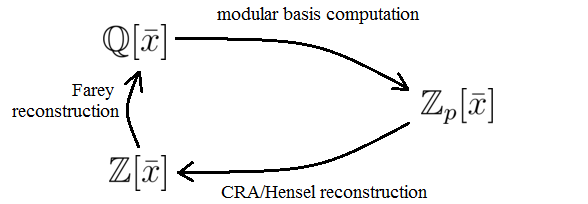
\includegraphics[scale=0.7]{reconstructionRelations.png}
  \caption{Modular basis computations and the reconstruction algorithms, relation between spaces \label{fig:bb_tests}}
\end{figure}

Before the modular reconstruction algorithms are discussed in detail, a new factor must be taken into account: there is a new problem associated with modular reconstructions.  Previously, working with the Groebner computation algorithms directly, there is no consideration for any external factors.  However, now the characteristics of a modular space must be considered.  In particular, the modular space must be a field; every element ${a}$ in the space (excluding the additive inverse, 0) must have a multiplicative inverse in the space i.e. a unique corresponding element ${a^{-1}}$ in the space such that ${a*a^{-1} = 1 = a^{-1}*a}$.  To ensure that this is the case, the positive integer ${m}$ in space ${\mathbb{Z}_m}$ must be a prime.

\begin{note}
  For the modular space ${\mathbb{Z}_m}$ to be a field, ${m}$ must be a prime.  

  \textbf{Proof:} If ${m}$ is prime, then every integer ${1 \leq k \leq m}$ has ${\gcd(k, m) = 1}$ and ${\exists \; s, \, t \in \mathbb{Z}}$ such that 
  \begin{equation*}
    s \cdot k + t \cdot m = \gcd(k, m) = 1
  \end{equation*}
  Hence, every nonzero ${k}$ has multiplicative inverse ${s \in \mathbb{Z}_m}$.  Therefore, ${\mathbb{Z}_m}$ is a field for ${m}$ prime, by definition of a field.

  Now, considering the alternative: if nonzero ${m}$ is composite, then ${\exists \; a, \, b \in \mathbb{Z}, a, \, b \neq 0, 1}$ such that ${m = a \cdot b}$.  Then, it follows that ${a \cdot b = 0 (\mod m)}$.  So, ${a}$ and ${b}$ would be zero divisors for the ring ${\mathbb{Z}_m}$.  However, a field is an integral domain (in which each nonzero element has an inverse relative to multiplication), and inverses are defined as having no zero divisors.  Therefore, ${\mathbb{Z}_m}$ is not a field for ${m}$ composite. \qed
\end{note} % CITE Durbin pg 129

Methods for reconstruction from the prime modular integers to the integers, and then from the integers to the rationals, are detailed in the following chapter.  The methods which will be examined are Garner's Algorithm for Chinese Remainder computation and Hensel's algorithm, for building back from the prime modular integers to the integers; and Farey rational reconstruction for building back from the integers to the rationals.

\chapter{Modular Homomorphisms and Reconstruction}

Post processing in modular polynomial space requires reconstruction back to ${\mathbb{Z}[x_1, \ldots, x_n]}$, which is done through either the Chinese Remainder Algorithm (henceforth the CRA) or Hensel's Algorithm, which will be described below.  Subsequent reconstruction from the integers to the rationals is done using an algorithm similar to Farey rational reconstruction, which is also described below.  This chapter also discusses a new difficulty which arises when attempting to reconstruct - the idea of \textbf{lucky primes}. 

\section{Chinese Remainder Theorem} 

The CRA is a method for reconstruction of an integer (or set of integers); it requires a set of modular images over various primes, which, combined provide a mixed-radix representation of the integer being reconstructed.  

\subsection{Mixed Radix Representation}

In general, when numbers are considered as representations of a sum of values, this is in terms of a set of multiples of successive powers of a particular base.  The general definition is as follows:

\begin{defn}\label{Basic defn}
  For a value ${x \in \mathbb{Z}}$ in base ${b > 0,\, b \in \mathbb{Z}}$,
  \begin{equation*}   x = \sum\limits_{i = 0}^{n}{a_ib^i}     \end{equation*}
  For ${\{a_i\} \subset \mathbb{Z},\, 0 \leq a_i < b \; \forall a_i}$ 
\end{defn}

This representation is \textbf{single-radix}, since it uses a single radix (or base) to represent a number.  \textbf{Mixed-radix representation} is a similar idea; however, instead of a linear combination of successive powers of a particular base, it is built from a linear combination of products of successive multiple "bases" - there is not a consistent base for all numerical positions.  The idea is similar in that the sequence of terms in the sum are in the base of a multiple of the previous base, however the factor of this multiple is not constant.  

One classic demonstrative example is in representing time: to tell the day, this is a sum of seconds and minutes and hours and days, each of which is a different successive radix.  There is no consistent base across all these terms, however each base is a multiple of the previous one (60 seconds in a minute, 60 minutes in an hour, 24 hours in a day, 7 days in a week).     

The CRA uses the various modular images provided to iteratively construct a mixed-radix representation of the original value, in order to perform the reconstruction.


\subsection{Chinese Remainder Algorithm} 

The Chinese Remainder Problem made its earliest appearance in the 3rd century, in the book \textit{Sunzi's Mathematical Classic}, by Sun Tzu, a Chinese mathematician.  The description of the algorithmic solution to this problem was then described in the 6th century by another mathematician, Aryabhata.  Gauss also described this, when he introduced the concept of modular congruences, in his 1801 book \textit{Disquisitiones Arithmeticae}.  
% (this is cited from elwiki, but I'm sure it's in another, more socially acceptable source)   CITE

\noindent The \textit{Chinese Remainder Problem} can be stated as: 
\begin{addmargin}[2em]{2em}% 2em left and right
  Given a set of moduli ${\{m_i\} \subset \mathbb{Z}}$ and corresponding residues ${\{u_i\} \subset \mathbb{Z}}$, where ${i}$ ranges from 0 to ${n \in \mathbb{Z}}$; find an integer ${u}$ which satisfies the congruences
  \begin{equation*}
    u \equiv u_i \mod m_i\, ; \quad \forall i \in [0, n]
  \end{equation*} 
\end{addmargin}

The algorithm for solving this problem is essentially an inversion of the modular homomorphism (i.e. rebuilding the original integer ${u}$ from various of its modular images).  The Chinese Remainder Problem specifies \textit{an} integer; however there are conditions under which the solution to this problem is unique.   

\begin{theorem}\label{Chinese Remainder Theorem}
  Let the set ${\{m_i\} \subset \mathbb{Z}}$, where ${i \in [0, n] \subset Z}$, be a set where all elements are pairwise relatively prime i.e.
  \begin{equation*}
    gcd( m_j, m_k) = 1 \; \forall \, j \neq k
  \end{equation*}
  and let ${\{u_i\} \subset \mathbb{Z}_{m_i}}$ be the corresponding residues.  Then, for any fixed integer ${a \in \mathbb{Z} \; \exists}$ a unique integer ${u \in \mathbb{Z}}$ which satisfies the following conditions:
  \begin{itemize}
    \item ${a \leq a + m}$, where ${m = \prod_{i=0}^{n}m_i}$
    \item ${u \equiv u_i \mod m_i\, ; \forall i \in [0, n] \subset \mathbb{Z}}$
  \end{itemize}  
\end{theorem}

The process of solving the Chinese Remainder Problem is generally done using Garner's algorithm.  Developed in the 1950s, this algorithm reconstructs the unique number satisfying the modular congruences provided (provided there is a unique solution, satisfying the conditions as given by the Chinese Remainder Theorem) by representing it in mixed-radix form.  

Garner's Chinese Remainder Algorithm is given below in pseudocode.

\begin{algorithm}[H]
\caption{Garner's Algorithm for Chinese Remainder}\label{CRA}
\begin{algorithmic}[1]
\Input $\; \; $ set of pairwise relatively prime moduli ${\{m_i\} \subset \mathbb{Z}}$, and corresponding residues ${u_i \in \mathbb{Z}_{m_i}}$
\Output unique integer ${u \in \mathbb{Z}_m}$ (with ${m = \prod_{i=0}^{n}m_i}$), such that the congruences are satisfied ${\forall i}$  
\Procedure{CRA\_int}{}
\State // first: compute the modular inverses required
\State // this will be using a procedure $inverse( a, q)$ which computes ${a^{-1} \mod q}$
\For{ $k$ from 1 to $n$}
  \State $curTerm \gets curTerm * m_k$
  \State $curProds_k \gets curTerm$\\
  \State $\gamma_k \gets reciprocal( curTerm, m_{k+1})$
\EndFor\\

\State // now need to compute the $v$'s (the mixed-radix coefficients)\\
\State $curTerm \gets 0$

\For{ $k$ from 0 to $n$}
  \State $v_k \gets ((m_k - curTerm) * \gamma_k) \mod m_k$
  \State $curTerm \gets curTerm + curProds_k * v_k$
\EndFor\\

\State // now, compute $u$; the sum of the mixed-radix representation

\State $u \gets 0$
\For{ $k$ from 0 to $n$}
  \State $u \gets u + v_k * curProds_k$
\EndFor\\\\

\Return $u$
\EndProcedure
\end{algorithmic}
\end{algorithm} 

A demonstrative example of the CRA is included below, over the integers.  Note that the process is the same for polynomials; every coefficient in the polynomial is reconstructed via the CRA.

\begin{example}\label{CRA}
  Consider the following modular equivalences:
  \begin{eqnarray*}
    x &=& 2 \mod 3\\
    x &=& 3 \mod 7\\
    x &=& 0 \mod 2\\
    x &=& 0 \mod 5
  \end{eqnarray*}  
  Here, 2, 3, 5, 7 are all coprime; therefore, by the CRT, ${\exists}$ a unique solution modulo ${210 = 2 \cdot 3 \cdot 5 \cdot 7}$. 

  Now, calculate the components for the algorithm, following the pseudocode above.
  \begin{eqnarray*}
    M_2 = \frac{210}{2} = 105 \qquad ; \qquad \gamma_2 = (105)^{-1} \mod 2 = 1\\
    M_3 = \frac{210}{3} = 70 \qquad ; \qquad \gamma_3 = (70)^{-1} \mod 3 = 1\\
    M_5 = \frac{210}{5} = 42 \qquad ; \qquad \gamma_5 = (42)^{-1} \mod 5 = 3\\
    M_7 = \frac{210}{7} = 30 \qquad ; \qquad \gamma_7 = (30)^{-1} \mod 7 = 4
  \end{eqnarray*}

  Then, ${x}$ can be calculated as follows:
  \begin{eqnarray*}
    x &=& 0(M_2\gamma_2) + 2(M_3\gamma_3) + 0(M_5\gamma_5) + 3(M_7\gamma_7) \mod 210\\
      &=& 0 + 140 + 0 + 360 \mod 210\\
      &=& 500 \mod 210\\
      &=& 80
  \end{eqnarray*}

  So, the unique solution for ${x}$ as given by the modular images is 80.
\end{example}

This algorithm reconstructs an integer from the given modular images, over the modular integers modulo the product of the moduli.  However, this method is equally applicable to polynomials with integer coefficients.  In this case, the arguments to the procedure would be the same list of moduli, and the polynomial residues.  These residues can be thought of as sets of coefficient residues; each coefficient can be reconstructed essentially separately, using Garner's algorithm.  There will be no mixing of terms, as each coefficient (by definition of a polynomial) corresponds to a unique power product. 

An alternative to the Chinese Remainder Algorithm is Hensel's Algorithm.              

\section{Hensel's Algorithm}

The Chinese Remainder Algorithm (CRA) is one reconstruction method for rebuilding an integer post processing in over the modular integers.  However, one major drawback to the CRA is that it requires many modular images in order for the reconstruction to proceed.  As the size of the coefficients being rebuilt increases, so too does the number of images which have to be stored and iterated over.  It would be convenient to have a reconstruction method which requires fewer modular images in order to rebuild these larger coefficients.   

Hensel's algorithm is another reconstruction method, similar in aim to the CRA; however, unlike the CRA's mixed-radix representation it uses the idea of a single-radix, or ${p}$-adic representation.

\subsection{${p}$-adic Representation}

Recall the mixed-radix representation for integers as used in the CRA.  There is another representation technique for integers which instead uses a sum of successive products of a single prime.  Rather than reconstruction ending in a sum of the mixed radix representations such as in the CRA as
\begin{equation*}
  u = v_0 + v_1(m_0) + v_2(m_0m_1) + \ldots + v_n(\prod_{i=0}^{n-1}m_i)
\end{equation*}
for the moduli ${m_i}$, mixed-radix coefficients ${v_i}$, ${p}$-adic representation involves reconstructing ${u}$ as 
\begin{equation*}
  u = u_0 + u_1p + u_2p^2 + \ldots + u_np^n
\end{equation*}
for some prime ${p}$, ${n}$ such that ${p^{n+1} > 2 \mid u \mid}$, and ${u_i \in \mathbb{Z}_p\, i \in [0, n] \subset \mathbb{Z}}$.  This seems to be an identical approach to the regular single-radix representation; and indeed, if the positive modular representation is used, then the ${p}$-adic representation is equal to single-radix, over base ${p}$, for ${u}$ positive.  However, the symmetric representation makes more sense to use, as it allows the ${u}$ to be negative (consider, if positive modular representation was used, that none of the ${u_i}$ would be negative; and, since ${p^k > 0 \; \forall k \in \mathbb{Z}}$ for positive ${p}$ then ${u}$ can only be a sum of products of positive integers, which is always positive).  

Hensel's Algorithm reconstructs images using the ${p}$-adic representation, for a particular prime ${p}$.

\subsection{Hensel's Algorithm}

Here, consider that, similarly to the CRA, where extension of the methods to the polynomial case is simple, involving the application of the method to each of the coefficients of the method, Hensel's reconstruction algorithm can also be applied to solving modular congruences with polynomials instead of integers.  Here, the method presented will be for the univariate polynomial case.  

The idea is to have a reconstruction method equivalent to the CRA, but which only uses one prime image to invert the modular homomorphism ${\phi_p\; : \; \mathbb{Z}[x] \rightarrow \mathbb{Z}_p[x]}$.  Rather than starting with multiple images such as in the CRA, here we start with image ${u_0(x) \in \mathbb{Z}_p}$ of the requested solution ${u(x) \in \mathbb{Z}}$.

\begin{theorem}\label{hensel's lemma}
  Hensel's Lemma: Given ${p \in \mathbb{Z}}$ prime, and ${a(x) \in \mathbb{Z}[x]}$ univariate polynomial with integer coefficients; and given ${u^{(1)}(x),\, w^{(1)}(x) \in \mathbb{Z}_p[x]}$ relatively prime univariate polynomials over the ${p}$-modular integers such that
  \begin{equation*}
    a(x) \equiv u^{(1)}(x)w^{(1)}(x) \mod p
  \end{equation*}

  Then, for any integer ${k \geq 1 \; \exists \; u^{(k)}(x),\, w^{(k)}(x) \in \mathbb{Z}_{p^k}[x]}$ such that 
  \begin{equation*}
    a(x) \equiv u^{(k)}(x)w^{(k)}(x) \mod p^k
  \end{equation*}
  and ${u^{(k)}(x) \equiv u^{(1)}(x) \mod p}$, ${w^{(k)}(x) \equiv w^{(1)}(x) \mod p}$. 

  Note: the proof is not given here; refer to CN for the full proof.
\end{theorem}           

The Hensel construction (given by Hensel's lemma above) is built from the linear ${p}$-adic Newton's iteration.  The idea essentially amounts to iteratively building up the ${p}$-adic representation of ${u}$ from the first image given (rather than computing many separate images over different moduli as in the CRA).  The problem from the outset is that there is not enough information from the single modular image to perform the next iterative reconstruction.  Extra information, usually in the form of a set of nonlinear equations which ${u(x)}$ must satisfy, is also provided to the algorithm.   

HOW MUCH SHOULD I REALLY EXPLAIN HERE ABOUT HENSEL  

Further details of the Hensel reconstruction are included in the discussion of the application of Hensel to Groebner bases specifically, as detailed by Arnold.

After the solution has been reconstructed from the modular integers to the integers, it must now be rebuilt to the rationals.

\section{Rational Reconstruction}

The original basis in these algorithms is assumed to be the polynomial extended rational numbers, ${\mathbb{Q}[x_1, x_2, \ldots, x_n]}$.  As such, postprocessing must be done on the output of the CRA/Hensel reconstruction to build the basis back to the polynomials over the rationals.  

One common approach for rational reconstruction is using the Farey rational map.  The method as described by B\"ohm is included below for explanation; this is also the method which was programmed in Maple as part of the modular methods.

The idea of rational reconstruction is to build back a number ${x \in \mathbb{Q}}$ from a modular image in ${\mathbb{Z}_p}$. 

Consider the rational number ${x \in \mathbb{Q}}$ which is being reconstructed.  Then, since ${x \in \mathbb{Q}}$ we have ${x = \frac{a}{b}}$ for some ${a,\,b \in \mathbb{Z}}$ and some integer ${N \geq 2}$, with ${\gcd(a, b) = 1,\, \gcd(b, N) = 1}$.
Then
\begin{equation*}
  x_N = \left(\frac{a}{b}\right)_N = (a + N\mathbb{Z})(b + N\mathbb{Z})^{-1} \in \frac{\mathbb{Z}}{N\mathbb{Z}}
\end{equation*}   

Note that ${x_N}$ is a modular integer; as such, it is an equivalence class of rationals modulo ${N}$, i.e. the infinite set of rationals ${\frac{a}{b}}$ which are all equal modulo ${N}$.  This set is a member of the fraction field ${\frac{\mathbb{Z}}{N\mathbb{Z}}}$, which itself is isomorphic to ${\mathbb{Z}_N}$.

This approach to rational reconstruction uses the idea of a Farey rational map, which is defined (using B\"ohm's notation) for an integer ${B > 0}$ as:
\begin{equation*}
  F_B = \left\{\frac{a}{b} \in \mathbb{Z}\; : \; \gcd(a, b) = 1,\, 0 \leq a \leq B,\, 0 < |b| \leq B\right\}
\end{equation*}
Basically, the Farey rational map contains all the rational numbers (representatives of the equivalence classes of rational numbers, i.e. fractions in lowest terms, where the GCD of the numerator and the denominator is 0) where the absolute value of the numerator and denominator range from 0 (1 for the denominator) to ${B}$.  This set will be finite for a finite ${B}$.

Then, define for ${m \in \frac{\mathbb{Z}}{N\mathbb{Z}}}$:
\begin{equation*}
  \mathbb{Q}_{N, m} = \left\{\frac{a}{b} \in \mathbb{Q}\; : \; \gcd(a, b) = 1,\, \gcd(b, N) = 1,\, \left(\frac{a}{b}\right)_N = m\right\}
\end{equation*}
the set of rational numbers which are congruent to ${m}$ modulo ${N}$.  

As B\"ohm states, the set ${\mathbb{Q}_N}$ can be expressed as the union of all the ${\mathbb{Q}_{N, m}}$ where ${m}$ ranges from 0 to ${N - 1}$.  This is fairly intuitive; each set is the equivalence class of ${m}$ modulo ${N}$ over the rational numbers; as such, the set of all possible ${m}$ ranges from 0 to ${N - 1}$ inclusive, as this is the range of the ${N}$-modular integers.  Therefore, there are ${N}$ distinct equivalence classes, and the union of these sets is the entire set ${\mathbb{Q}_N}$ itself (as equivalence classes, by definition, form a partition of the set the relation is defined over; here, the relation is modulo ${N}$, which is an equivalence relation).  

If ${B}$ is an integer where ${B \leq \sqrt(\frac{N - 1}{2})}$, then the \textbf{Farey map} can be defined as the mapping
\begin{equation*}
  \phi_{B, N}:\; F_B \bigcap \mathbb{Q}_N \rightarrow \frac{\mathbb{Z}}{N\mathbb{Z}},\quad \frac{a}{b} \rightarrow \left(\frac{a}{b}\right)_N
\end{equation*}

This mapping is well-defined and injective (as stated by B\"ohm).  This returns the original rational ${x}$.  To maximize image returned from this mapping with respect to ${N}$, choose ${B}$ to be the largest possible value for the ${N}$ specified.

The following algorithm calculates the Farey preimage as discussed in the B\"ohm paper; it returns the inverse image ${\phi_{B, N}^{-1}(y)}$ if ${y}$ is in the image of the Farey map with respect to the mapping ${\phi}$; if this value cannot be computed (for example, if the value attempting to be reconstructed does not fit the acceptance criteria, essentially amounting to the inverse image of modular integer ${N}$) then \texttt{false} is returned to indicate to the user that there was an error in the computation, and that the value used to attempt the calculations was a "bad prime" with respect to this rational reconstruction.

\begin{algorithm}[H]
\caption{Farey Reconstruction}\label{farey}
\begin{algorithmic}[1]
\Input $\quad$Integers $\; N \geq 2 \;$ and $\; 0 \leq r \leq N - 1$
\Output $\texttt{false} \,$or a rational number$\, a/b \,$ with$\, gcd(a, b) = 1,\, gcd(b, N) = 1,$ $\; a/b \equiv r $ mod $ N, \, 0 \leq a \leq \sqrt{(N-1)/2}, \, 0 \leq \abs{b} \leq \sqrt{(N-1)/2}.$ 
\Procedure{FareyRecon}{}
\State $a \gets [ N, r]$
\State $b \gets [ 0, 1]$
\State $i \gets 0$
\While{ $2a_{i+2}^2 \geq N-1$ } 
  \State $i \gets i + 1$
  \State $q \gets \text{floor}( a_i / a_{i+1})$
  \State $a_{i+2} \gets a_i - qa_{i+1}$
  \State $b_{i+2} \gets a_i - qb_{i+1}$
\EndWhile\\  
\If { $2b_{i+2}^2 < N-1$ \textbf{ and} $gcd( a_{i+2}, b_{i+2}) = 1$ } 
  \State \quad \Return $[ a_{i+2}, b_{i+2}]$
\Else 
  \State \quad \Return false
\EndIf
\EndProcedure
\end{algorithmic}
\end{algorithm}

One problem associated with the reconstruction techniques (both from modular integers to integers, and from integers to rationals) is the concept of \textbf{lucky primes}, as mentioned previously.    

\section{Lucky Primes}

Naively, it would seem that using the smaller primes would make this process more efficient - smaller primes would mean a smaller upper bound on the coefficients, and therefore a more computationally efficient basis computation.  However, not every prime is valid for use in the reconstruction.  This can be seen directly in the rational reconstruction algorithm; some primes may return an invalid fraction if their magnitude is insufficient compared to the other inputs to the function.  

The CRA and Hensel's algorithm also have the potential for "bad" primes - this would be primes for which algebraic information is lost during processing in this modular space.  If during a computation there is a value for which this prime is a divisor, then this term would vanish when the basis is taken modulo the prime - then, this term can no longer be reconstructed, as it will no longer be present in any of later computations.

In Arnold's paper, she defines lucky primes as primes for which "we do not lose too much algebraic information" about ideal ${I \subseteq \mathbb{Q}[X]}$ when considering the ideal modulo prime p, ${I_p \subseteq \mathbb{Z}_p[X]}$.  For the modular lifting via CRA/Hensel, the required algebraic information is the set of leading terms of Groebner basis ${G}$ for ${I}$.

Formally: % CITE
\begin{defn}\label{Lucky Primes}
  A prime integer ${p}$ is a \textbf{lucky prime} for ideal ${I \subseteq \mathbb{Q}[X]}$ ${\iff}$ ${Lp(G) = Lp(G_p)}$
\end{defn}

\begin{note}
  A note on notation, with respect to the component parts of a polynomial.  Here, Arnold's notation will be adopted.  Note that in several other papers referenced, the notation may not match precisely, and some translation is necessary to determine which of their notation is equivalent to which of Arnold's notation.  Here, Arnold's notation will be used throughout for consistency.  

  In this case, the Groebner basis is considered over the Noetherian ring ${R = \mathbb{Q}[X]}$ 
  \begin{itemize}
    \item ${lp(f)}$ is the leading power product of polynomial ${f \in R}$
    \item ${lc(f)}$ is the leading coefficient of polynomial ${f \in R}$ (i.e. the coefficient of the leading power product)
    \item ${lt(f)}$ is the leading term of polynomial ${f \in R}$.  This is can be computed as ${lt(f) = lc(f)lp(f)}$ 
    \item ${Lp(R) = \{lp(f) \mid f \in R\}}$ is the set of leading power products of ${R}$
    \item ${Lc(R) = \{lc(f) \mid f \in R\}}$ is the set of leading coefficients of ${R}$
    \item ${Lt(R) = \{lt(f) \mid f \in R\}}$ is the set of leading terms of ${R}$
  \end{itemize}
\end{note}

Considering the definition of lucky primes as above, this relies on the Groebner basis having already been computed for ideal ${I}$.  This leads to some difficulties in using this definition to determine whether or not a prime is lucky for the actual computation - if the luckiness can only be determined post-processing with a comparison to the actual Groebner basis, this makes the luckiness checking fairly useless.  Instead, it would be convenient to be able to tell if a prime is lucky before performing the entire computation and checking if it results in a valid basis at the end.  

There are two alternate, more applicable definitions of lucky primes which will be considered in this case.

\subsection{Hilbert and Pauer}

The first definition to be considered is as given by Pauer in his paper on prime luckiness applied to Groebner bases.  

\begin{defn}\label{Pauer lucky}
  A prime ${p}$ is \textbf{Pauer lucky} for ideal ${I}$ if it does not divide any leading coefficient of any polynomial in ${G}$ the reduced Groebner basis of ${I}$.
\end{defn}

However, again, this relies on the true Groebner basis having been previously computed which essentially nullifies the algorithm. 

TODOOOOOO

Considering lucky primes, the effects of performing the computations with a bad prime varies on the algorithm in use. 

\subsection{Reconstructions: Lucky Prime Efficiency Comparison}

Although Hensel's algorithm is more efficient in terms of the number of images stored in compared with the CRA, it does have its drawbacks.  In particular, when considering "vulnerability" to bad primes, the CRA can simply discard a bad modular image; however the Hensel algorithm, since it relies on only one prime and images over its successive power products, has a harder time dealing with these.  The CRA can easily detect a bad prime (so long as the first prime used is lucky) by comparing the number of terms in the polynomials or taking the modulus of the previous basis with respect to this new prime to ensure the same answer is achieved.  Then, this modular basis computation has been wasted, however the reconstruction can continue with a new prime.  The Hensel lifting, on the other hand, cannot detect bad primes as easily, since all its computations are based on this prime and it has no other primes to compare results with.  As such, bad primes are not effectively found until the computation is done and the correctness of the output can be verified.  If the prime was bad, the entire Hensel process was a computational waste of time; as such, when using Hensel, the preemptive removal of bad primes is paramount.



Now that the reconstruction algorithms have been introduced, they can be applied to the Groebner basis computations. 


\chapter{Modular Groebner Basis Reconstruction}

The modular reconstruction methods introduced in the previous chapter can be applied to Groebner basis computations; they can be used in conjunction with the regular basis algorithms, over modular prime fields.  In the non-modular case, the algorithm (Buchberger, F4, or otherwise) can be applied directly to the supplied ideal basis, producing a single result which is the desired basis.  However, in the modular reconstruction case, there are added computations.  

For the CRA, various basis computations must be performed, each for the basis in a prime modular field, one for each of the primes necessary for the reconstruction.  The idea is that the various modular basis computations, coupled with the reconstruction code and the rational reconstruction will be more efficient (in both time and/or space) than the algorithm over the polynomial extended rational space, because of the elimination of the intermediate expression swell.  

For the CRA case, the algorithm proceeds iteratively:
\begin{enumerate}
  \item pick a good prime ${p_n}$
  \item perform a Groebner basis computation over ${\mathbb{Z}_{p_n}}$ coefficient field, returning ${G_{p_n}}$
  \item then, run the CRA reconstruction with ${G_{p_n}}$ and the basis ${G_{p_1p_2 \cdots p_{n-1}}}$, to build the basis ${G_{p_1p_2 \cdots p_{n-1}p_n}}$ 
  \item then, do the rational reconstruction on the new basis ${G_{p_1p_2 \cdots p_{n-1}p_n}}$ 
  \item the termination condition is if the rational reconstruction result for ${G_{p_1p_2 \cdots p_{n-1}p_n}}$ succeeds, and is identical to the reconstruction of ${G_{p_n}}$
  \item if the termination condition is not reached, then find another prime ${p_{n+1}}$ and repeat the process
\end{enumerate}

Hensel's algorithm proceeds similarly.  In this case, the algorithm is presented as in the Pauer paper, which is also referenced and explained by Arnolds.  Since the Hensel algorithm requires more initial information in order to proceed with the lifting (as stated in the explanation of the Hensel algorithm above, usually a system of equations which the initial modular image must satisfy).  

Here, the process of the ${p}$-adic lifting is as summarized in the Arnolds paper.  

Given an ideal ${I_{p} = \; <\bar f_1, \ldots, \bar f_r> \; \subseteq \mathbb{Z}_{p}[\bar x]}$, the goal is to lift this to ${I_{p^i} = \; <\bar f_1, \ldots, \bar f_r> \; \subseteq \mathbb{Z}_{p^i}[\bar x]}$, for some positive integer power ${i}$ of ${p}$.  Take ${F = \{f_1, \ldots, f_r\}}$ the set of generating polynomials for the ideal ${I}$.  

This procedure also begins with the assumption that the prime ${p}$ chosen is lucky for this ideal.

The steps of the process for lifting from a reduced Groebner ${G_p}$ for ${I_p}$ to monic reduced Groebner basis ${G_{p^i}}$ for ${I_{p^i}}$ is as described in the Arnolds paper.

\begin{enumerate}
  \item Compute ${G_p}$ for lucky prime ${p}$.  Also, consider the sets ${G_p}$ and ${F}$ (as above) as column vectors, and calculate the transformation matrix ${Z^{(1)}F \equiv G_p \mod p}$
  \item Then similarly, for ${i}$, it is necessary to find the matrices ${Z^{(i)}F \equiv G^{(i)} \mod p^i \quad}$ and ${\quad G^{(i)} \equiv G_p \mod p}$.  From this step, the reduced monic basis ${G_{p^i}}$ for ${I_{p^i}}$ can be computed.
  \item This computation is done recursively (iterating up to ${i}$); from the ${Z^{(i-1)}}$ and ${G_{p^{i-1}}}$ for step ${i-1,\, i > 1}$, first compute intermediate matrices ${Z', G'}$ where
  \begin{equation*}
    Z^{(i)} = Z^{(i-1)} + p^{i-1}Z'
  \end{equation*}
  and similarly
  \begin{equation*}
    G^{(i)} = G^{(i-1)} + p^{i-1}G'
  \end{equation*}
  with ${F^{(i)},\, G^{(i)}}$ defined as above: ${Z^{(i)}F \equiv G^{(i)} \mod p^i \quad}$
  This is done by solving the resultant modular congruence in terms of the intermediate matrices ${Z'}$ and ${G'}$:
  \begin{equation*}
    (Z^{(i-1)} + p^{i-1}Z')F \equiv G^{(i-1)} + p^{i-1}G'\mod p^i \quad
  \end{equation*}
  \item To solve this congruence, use Pauer's technique as presented in the Arnolds paper; using the originally computed modulo-${p}$ Groebner basis ${G_p}$ to reduce ${G'}$ to a new set ${G''}$ where there are no overlapping power products between ${G''}$ and ${Lp(G_p)}$.  \\ Consider ${M}$ the matrix of polynomials used in this reduction of ${G'}$.  Then, ${G' = MG_p + G''}$.\\ Take ${Z'' = Z' - MZ^{(1)}}$, with ${Z^{(1)}}$ as defined for the base case above.  These new sets ${Z'',\, G''}$ are solutions for the congruence above.
  \item Compute ${G_{p^i}}$ the reduced monic Groebner basis of ${I_{p^i}}$, with ${G_{p^i} = G^{(i)} = G_{p^{i-1}} + p^{i-1}G'}$
  \item Now that the ${G_{p^i}}$ has been computed, check the termination condition: apply Farey reconstruction (or another method of rational reconstruction) to rebuild the basis over the rationals.  If this result is the same as the rebuilt basis for ${i-1}$ then the result has stabilized, and the algorithm terminates.  Otherwise, repeat this process for ${i+1}$.
\end{enumerate}      

Note that in either case (CRA or Hensel), the result must be verified for correctness before the computed basis can be returned as the solution.  This check is necessary as there is not a guarantee that the prime (or first prime in the CRA) over which the bases were computed were actually lucky primes.  This check is fairly straightforward: the S-polynomials for every pair of polynomials in the computed basis ${G}$ must be verified to be equal to zero.  If this check fails, then the algorithm must restart from the outset.  Note that the Hensel approach is more vulnerable to bad primes, as seen above.

Now that the theory of the methods has been discussed, the algorithms can be implemented and the efficiency tested.  In this case, they were implemented using the Maple computer algebra system.

\section{Maple}

To test the comparative efficiency of the modular reconstruction algorithms and the direct basis computation, the algorithms were implemented in Maple.  Therefore, the tests were performed relative to the built-in Maple Groebner package.  Similar tests could be performed in other symbolic languages testing against their built-in Groebner functionality, such as Mathematica, Python's sympy, etc.  Some technical details of the Maple Groebner basis package are discussed below:

There are various versions of the basis computation algorithms available in the Maple Groebner package; these include the classic Buchberger algorithm, the F4 algorithm implemented in Maple (maplef4), and the F4 algorithm implemented as an external C library, FGB.  In Maple, when a Groebner basis computation is performed, this requires a call to the Basis command in the Groebner package - the arguments specified are the basis for the current ideal, the monomial ordering used, and optional arguments specifying the algorithm type used, and the characteristic prime if working over a modular prime coefficient field.   

The current most efficient built-in basis algorithm in Maple is the FGB algorithm.  This is an efficient, optimized implementation of the Faugere F4 algorithm; it is written in C which also increases the efficiency of the algorithm.  However, this method suffers from lack of implementation of various options: for instance, it cannot be used for any monomial ordering other than degree-based (it does not support lex orderings).  In addition, when using the characteristic prime option to specify a modular field, FGB does not support primes greater than ${2^{16}}$, which becomes an issue when calling the modular reconstruction methods.  In these cases, various prime images are required, and this number increases as the primes are smaller.  In addition, smaller primes leads to the a higher probability of the primes being bad primes.  The comparative effect of efficiency between using more, smaller primes and fewer, larger primes will be examined in the results section.  However, note here that primes used for CRA/Hensel here were in the neighbourhood of ${2^{31}}$; in this way, the coefficients are guaranteed to be integers smaller than the maximum word space of the system, which means that the computations can be performed whilw keeping the product of integers in the range which can be represented in hardware on a 64-bit machine (as was available for these tests).  However, when using FGB the primes were restricted to the smaller size.

The more efficient algorithms also cause issues for Hensel construction; Hensel requires another optional argument in the basis computation, output=extended, which specifies that the basis computation should the Syzygy matrix, ${Z^{(1)}}$ as discussed above in the description of the Hensel Groebner approach from the Arnolds paper.  The Hensel lifting algorithm itself is implemented with this matrices as input.  However, the functionality of Faugere's algorithm is such that the intermediate matrices are not computed, and therefore output=extended is not an option for the non-Buchberger algorithms.  

The algorithm selected for the Groebner basis computation does not change the process of the reconstruction; this is an external call.



The methodology and results of the tests are presented and discussed in the following chapter.

\chapter{Methodology and Results}

In order to obtain a wide range of data to have the potential to make conclusions, a set of problems must be constructed, representing the range of Groebner basis problems (a set of total degree, number of polynomials, coefficient size, integers/rationals, number of terms in the polynomial) was constructed and timing tests run on them with the various constructed algorithms, in order to compare.  These problems are included 

PSEUDOCODE OF THE MAPLE CALL

The results of the various algorithms running, with the various homomorphism implementations, were compared in terms of computational time.  

\noindent \textbf{Technical Details:}

The time computations were run on a VM server hosted at coscvm22.cs.laurentian.ca.  This VM was for the express purpose of these simulations, and as such there were no other user processes running on it.

\noindent \textbf{OS:} 64-bit Ubuntu 14.04\\
\textbf{Cores:} 6 logical cores\\
\textbf{Maple install:} 64-bit Maple 15

The timings were run with the Maple \texttt{time()} command.  This command returns the total CPU time used since the Maple session has started.  The time returned only includes the time for which maple was running, and not that during which the CPU was running other processes.  This is a more accurate measure of the time taken for the basis computation (as opposed to, for example, the bash \texttt{time} command).

Various problems were selected, in order to represent a range of each of the main factors affecting complexity of Groebner basis computations, as discussed above: degree, number of variables, and initial coefficient size.  There are also a range of problems in terms of the number of generating polynomials in the initial ideal, and the sparsity of these polynomials (i.e. the number of nonzero coefficients in the polynomials).  This range is qualitatively described in the table below.

TABLE HERE

The above problems were attempted with the various algorithms (Buchberger, MapleF4, and FGB) and methods (Hensel, CRA, and regular Maple).  The overall results are summarized in the following table; these are the overall Maple timings for the problems running on the server.  Details of how the running was implemented are included in Appendix \ref{appendix:running}.

\section{Raw Data}

-- here is the data

\singlespacing
\refstepcounter{Table}
\begin{center}
  \begin{tabular}{| l || r | r | r || r | r || r | r ||}
  \multicolumn{8}{l}{\textbf{Table \theTable}: total timings for select problems}\\
  \hline 
  & \multicolumn{3}{c}{Buchberger} & \multicolumn{2}{c}{MapleF4} & \multicolumn{2}{c}{FGB} \TBstrut\\
  \hline
  Problems & CRA (s) & Hensel (s) & Maple (s) & CRA (s) & Maple (s) & CRA (s) & Maple (s)\\
  % Parameter & Average Relative Error & Variance of the Error \TBstrut \\ 
  \hline\hline
  arnborg1 & 0.723 & 18.969 & 0.423 & 0.532 & 0.312 & 0.1 & 0.036\\
  arnborg2 & 36.884 & \textbf{\textit{DNF}} & 14.812 & 9.661 & 3.673 & 0.56 & 0.072\\
  arnborg3 & 0.336 & 2340.014 & 0.2 & 0.264 & 0.139 & 0.159 & 0.036\\
  arnborg5 & 3.436 & \textbf{\textit{DNF}} & 1.408 & 3.436 & 1.072 & 0.367 & 0.052\\
  forsman1 & 0.192 & 0.891 & 0.084 & 0.239 & 0.136 & 0.063 & 0.028\\
  forsman2 & 0.028 & \textbf{\textit{DNF}} & 0.015 & 0.032 & 0.016 & 0.052 & 0.023\\
  forsman3 & 0.068 & \textbf{\textit{DNF}} & 0.108 & 0.068 & 0.028 & 0.059 & 0.024\\
  forsman4 & 0.804 & \textbf{\textit{DNF}} & 0.243 & 0.468 & 0.099 & 0.129 & 0.043\\
  katsura7 & 282.393 & \textbf{\textit{DNF}} & 24.604 & 153.189 & 38.533 & 16.554 & 0.496\\
  hellin & 1.795 & 1.944 & 0.12 & 2.253 & 0.116 & 1.977 & 0.039\\
  kiyoshi5 & 1.128 & 1.212 & 0.016 & 1.152 & 0.024 & 2.321 & 0.044\\
  caprasse & 0.416 & 10.684 & 0.283 & 0.384 & 0.204 & 0.572 & 0.053\\
  mike2 & 38.936 & \textbf{\textit{DNF}} & 5.8 & 25.533 & 5.06 & 2.669 & 0.105\\
  czap27 & 247.147 & \textbf{\textit{DNF}} & 34.236 & 66.784 & 11.92 & 4.88 & 0.283\\
  czap33 & 0.443 & 1.176 & 0.035 & 0.4 & 0.08 & 0.519 & 0.04\\
  czap34 & 1.72 & 1.924 & 0.079 & 2.04 & 0.132 & 1.9 & 0.051\\
  czap41 & 20.956 & 89.82 & 0.456 & 27.987 & 1.08 & 16.964 & 0.264\\
  trav1 & 0.028 & 0.1 & 0.028 & 0.04 & 0.059 & 0.053 & 0.04\\
  cassou\_POSSO & 6.694 & \textbf{\textit{DNF}} & 2665.155 & 2.204 & 0.856 & 0.28 & 0.041\\
  cyclic6 & 37.444 & \textbf{\textit{DNF}} & 14.949 & 10.076 & 3.636 & 0.527 & 0.065\\
  cyclic7 & \textbf{\textit{DNF}} & \textbf{\textit{DNF}} & \textbf{\textit{DNF}} & \textbf{\textit{DNF}} & \textbf{\textit{DNF}} & \textbf{\textit{DNF}} & \textbf{\textit{DNF}}\\
  cyclic8 & \textbf{\textit{DNF}} & \textbf{\textit{DNF}} & \textbf{\textit{DNF}} & \textbf{\textit{DNF}} & \textbf{\textit{DNF}} & \textbf{\textit{DNF}} & 123.924\\
  hcyclic8 & \textbf{\textit{DNF}} & \textbf{\textit{DNF}} & \textbf{\textit{DNF}} & \textbf{\textit{DNF}} & \textbf{\textit{DNF}} & \textbf{\textit{DNF}} & \textbf{\textit{DNF}}\\
  katsura8 & \textbf{\textit{DNF}} & \textbf{\textit{DNF}} & \textbf{\textit{DNF}} & \textbf{\textit{DNF}} & \textbf{\textit{DNF}} & \textbf{\textit{DNF}} & \textbf{\textit{DNF}}\\
  katsura9 & \textbf{\textit{DNF}} & \textbf{\textit{DNF}} & \textbf{\textit{DNF}} & \textbf{\textit{DNF}} & \textbf{\textit{DNF}} & \textbf{\textit{DNF}} & \textbf{\textit{DNF}}\\
  katsura10 & \textbf{\textit{DNF}} & \textbf{\textit{DNF}} & \textbf{\textit{DNF}} & \textbf{\textit{DNF}} & \textbf{\textit{DNF}} & \textbf{\textit{DNF}} & \textbf{\textit{DNF}}\\
  repulso1 & \textbf{\textit{DNF}} & \textbf{\textit{DNF}} & \textbf{\textit{DNF}} & \textbf{\textit{DNF}} & \textbf{\textit{DNF}} & \textbf{\textit{DNF}} & \textbf{\textit{DNF}}\\
  repulso2 & \textbf{\textit{DNF}} & \textbf{\textit{DNF}} & \textbf{\textit{DNF}} & \textbf{\textit{DNF}} & \textbf{\textit{DNF}} & \textbf{\textit{DNF}} & \textbf{\textit{DNF}}\\
  repulso3 & \textbf{\textit{DNF}} & \textbf{\textit{DNF}} & \textbf{\textit{DNF}} & \textbf{\textit{DNF}} & \textbf{\textit{DNF}} & \textbf{\textit{DNF}} & \textbf{\textit{DNF}}\\
  huygens3 & \textbf{\textit{DNF}} & \textbf{\textit{DNF}} & \textbf{\textit{DNF}} & \textbf{\textit{DNF}} & \textbf{\textit{DNF}} & \textbf{\textit{DNF}} & \textbf{\textit{DNF}}
  \\ % [1ex]
  \hline
  \end{tabular}
\end{center}
\doublespacing

\begin{note}
  The cells marked \textit{\textbf{DNF}} indicate that this problem "did not finish" (or ran out of mem -- RECHECK FILES); in these cases it was due to the Maple kernel running out of memory and crashing with a "not enough memory available" or "object too large" error.  
\end{note}

The table above shows various expected trends.

\begin{itemize}
  \item Across all algorithms, the FGB is the fastest, i.e. FGB Maple is faster than MapleF4 Maple and Buchberger Maple; the same result can be seen for the CRA
  \item  Maple is faster than the CRA, which in turn is faster than Hensel, on a per-algorithm basis
\end{itemize}

These trends can also be visually represented by way of bar graphs.

This style of analysis through testing of discrete examples mainly lends itself to representation via bar graphs.  Using specific examples, it is difficult to define a consistent ordering which can be represented well on a quantitative scale.  In this case there is also not a single independent variable; the 3 main factors (coefficient size, number and degree of variables) mean that a single linear x-axis does not make much sense.

\begin{figure}[H]
  \centering
  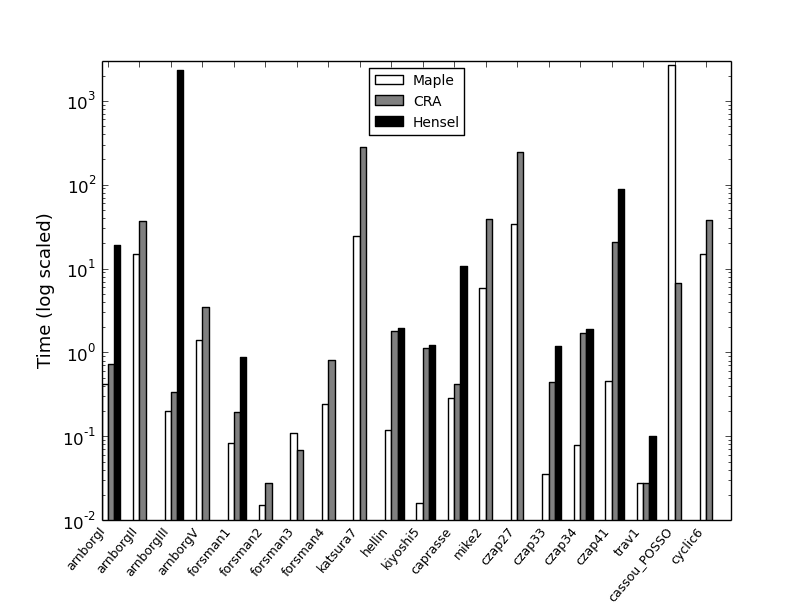
\includegraphics[scale=0.7]{bb_tests.png}
  \caption{Buchberger's algorithm, comparing the methods \label{fig:bb_tests}}
\end{figure}

This graph represents the timings of the methods run with the modular computations done using Buchberger's algorithm, with 32-bit primes.  The \textbf{DNF} Hensel problems show up as no Hensel bar on the chart.  The Hensel problems are seen to be slower than the CRA and Maple in every case in which Hensel terminates.  Similarly, the CRA seems to be consistently slower than the nonmodular Maple Buchberger, although there are 2 problems in this selection (forsman3 and cassou\_POSSO) in which the CRA was faster.

Similar graphs can be made for the MapleF4 and FGB algorithms.  Note, however, that there is no Hensel data in either of these cases; this is because the Hensel method requires the Buchberger's output=extended option, as discussed above.

\begin{figure}[H]
  \centering
  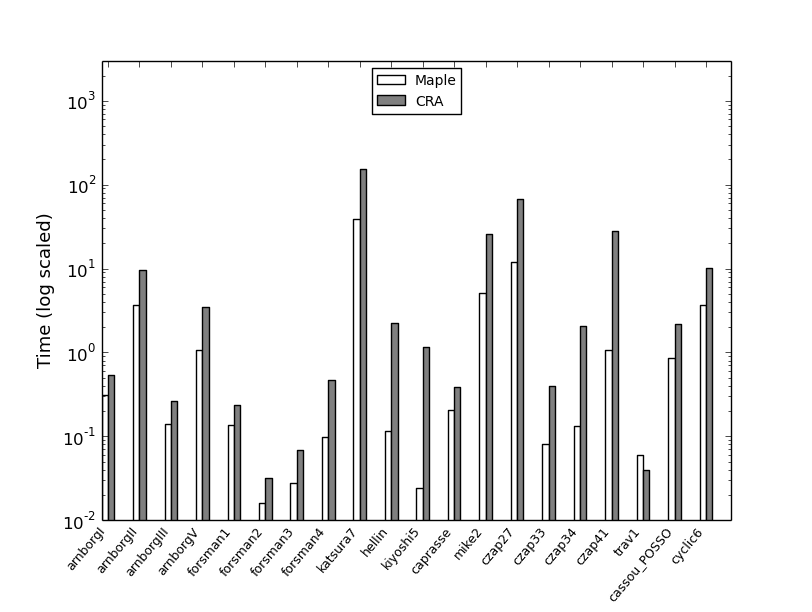
\includegraphics[scale=0.7]{f4_tests.png}
  \caption{MapleF4 algorithm, comparing the methods \label{fig:f4_tests}}
\end{figure}

\begin{figure}[H]
  \centering
  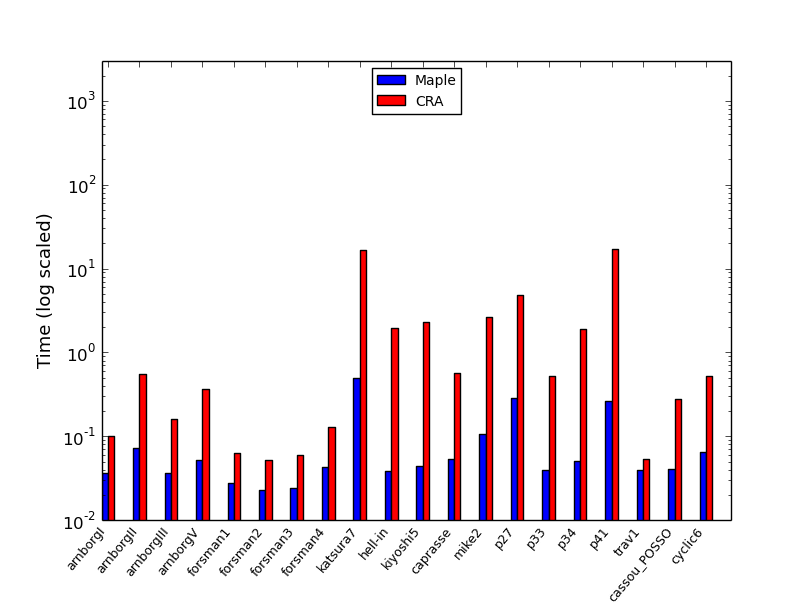
\includegraphics[scale=0.7]{fgb_tests.png}
  \caption{FGB algorithm, comparing the methods \label{fig:fgb_tests}}
\end{figure}

These graphs show the same trends as the Buchberger plot; the CRA is consistently slower than the nonmodular Maple in almost every case.  At this point, various conclusions could be drawn.

With regards to Hensel, this approach seems like a lost cause.  There are several points against it: for one, it seems to be slower in every case than the CRA and straight Maple approach in the Buchberger case.  In many cases, the algorithm did not terminate, while for the same problem it did terminate for other methods.  More importantly, Hensel can only be run with the modular basis computations using Buchberger's algorithm; since it relies on output=extended, it cannot make use of the faster basis computation algorithms available.  %lolol

However, although the CRA is still consistently slower than Maple, there are still potential efficiency improvements to the CRA.

\section{Potential Improvements to the CRA} 

The CRA computation can be broken down into stages:

\begin{enumerate}
  \item Modular basis computations, to generate modular images for reconstruction
  \item CRA reconstruction itself
  \item Farey reconstruction
\end{enumerate}

The modular basis computations are done using the Maple Groebner package, with whichever algorithm was selected; if this is the stage with the least time efficiency, then there is no clear approach to solving the problem.  This would mean that the Groebner package itself is not well-suited for the CRA, and fixing this would involve editing the Maple package itself, which cannot be done as a user as they do not provide the source code for their compiled libraries.

However, if the primary time cost is with either the CRA or Farey reconstruction, then this problem could potentially be addressed by other means.  Maple provides user the option of writing their own external libraries (in either C, Java, or FORTRAN).  In this case, approach would be to use C and the GMP MPZ library.  This is the GNU MultiPrecision package; the C MPZ library allows for manipulation of multiprecision integers as objects in C.  Using this, the CRA could be written in C and linked as an external library to Maple, in order to speed up the computation.  C is naturally faster than Maple, and allows for optimization using multithreading and other lower level functionality which is not available in Maple.  In addition, although the current code is using the Maple \texttt{iratrecon} reconstruction method, the Farey reconstruction could also be written in C and linked in similar to the CRA reconstruction.

The technical details of passing arguments and linking the library are included in \textbf{Appendix} \ref{appendix:running}.  

Profiling of the CRA runs was done to compare the proportion of total time during each stage of the CRA basis computations.  The results are included for all 3 algorithms in the tables below.  

The column headers are:
\begin{itemize}
  \item Mod Basis: time spent performing modular basis computations with the Groebner package (in seconds)
  \item Farey: time spent running rational reconstructions (in seconds)
  \item CRA: time spent running CRA reconstructions (in seconds)
  \item Total: total time for the CRA basis computation (sum of the above 3 terms) (in seconds)
  \item Images: the number of modular images which were required
\end{itemize} 

\singlespacing
\refstepcounter{Table}
\begin{center}
  \begin{tabular}{| l || r | r | r || r || r ||}
  \multicolumn{6}{l}{\textbf{Table \theTable}: CRA profiling, Buchberger's algorithm (32-bit primes)}\TBstrut\\
  \hline 
  Problems & Mod Basis (s) & Farey (s) & CRA (s) & \textbf{Total} (s) & Images \\
  % Parameter & Average Relative Error & Variance of the Error \TBstrut \\ 
  \hline\hline
   arnborg1 & 0.715 & 0.008 & 0 & 0.723 & 2 \\
   arnborg2 & 36.62 & 0.24 & 0.024 & 36.884 & 5 \\
   arnborg3 & 0.308 & 0.028 & 0 & 0.336 & 2 \\
   arnborg5 & 5.201 & 0.156 & 0.007 & 5.364 & 4 \\
   forsman1 & 0.168 & 0.02 & 0.004 & 0.192 & 2 \\
   forsman2 & 0.024 & 0.004 & 0 & 0.028 & 2 \\
   forsman3 & 0.204 & 0 & 0.012 & 0.216 & 2 \\
   forsman4 & 0.792 & 0.012 & 0 & 0.804 & 5 \\
   katsura7 & 272.61 & 9.407 & 0.376 & 282.393 & 13 \\
   hellin & 1.041 & 0.726 & 0.028 & 1.795 & 21 \\
   kiyoshi5 & 0.244 & 0.872 & 0.012 & 1.128 & 71 \\
   caprasse & 0.395 & 0.017 & 0.004 & 0.416 & 2 \\
   mike2 & 37.605 & 1.104 & 0.227 & 38.936 & 8 \\
   czap27 & 245.539 & 1.515 & 0.093 & 247.147 & 8 \\
   czap33 & 0.221 & 0.21 & 0.012 & 0.443 & 17 \\
   czap34 & 0.885 & 0.815 & 0.02 & 1.72 & 21 \\
   czap41 & 12.214 & 8.511 & 0.231 & 20.956 & 41 \\
   trav1 & 0.028 & 0 & 0 & 0.028 & 2 \\
   cassou\_POSSO & 6.622 & 0.068 & 0.004 & 6.694 & 11 \\
   cyclic6 & 37.187 & 0.233 & 0.024 & 37.444 & 5
  \\ % [1ex]
  \hline
  \end{tabular}
\end{center}

\refstepcounter{Table}
\begin{center}
  \begin{tabular}{| l || r | r | r || r || r ||}
  \multicolumn{6}{l}{\textbf{Table \theTable}: CRA profiling, MapleF4 algorithm (32-bit primes)}\TBstrut\\
  \hline 
  Problems & Mod Basis (s) & Farey (s) & CRA (s) & \textbf{Total} (s) & Images \\
  % Parameter & Average Relative Error & Variance of the Error \TBstrut \\ 
  \hline\hline
   arnborg1 & 0.52 & 0.012 & 0 & 0.532 & 2 \\
   arnborg2 & 9.376 & 0.279 & 0.006 & 9.661 & 5 \\
   arnborg3 & 0.24 & 0.024 & 0 & 0.264 & 2 \\
   arnborg5 & 3.252 & 0.18 & 0.004 & 3.436 & 4 \\
   forsman1 & 0.226 & 0.013 & 0 & 0.239 & 2 \\
   forsman2 & 0.028 & 0.004 & 0 & 0.032 & 2 \\
   forsman3 & 0.068 & 0 & 0 & 0.068 & 2 \\
   forsman4 & 0.456 & 0.008 & 0.004 & 0.468 & 5 \\
   katsura7 & 143.325 & 9.604 & 0.26 & 153.189 & 13 \\
   hellin & 1.312 & 0.929 & 0.012 & 2.253 & 21 \\
   kiyoshi5 & 0.37 & 0.766 & 0.016 & 1.152 & 71 \\
   caprasse & 0.368 & 0.016 & 0 & 0.384 & 2 \\
   mike2 & 24.343 & 1.129 & 0.061 & 25.533 & 8 \\
   czap27 & 65.269 & 1.444 & 0.071 & 66.784 & 8 \\
   czap33 & 0.234 & 0.146 & 0.02 & 0.4 & 17 \\
   czap34 & 1.219 & 0.793 & 0.028 & 2.04 & 21 \\
   czap41 & 19.183 & 8.666 & 0.138 & 27.987 & 41 \\
   trav1 & 0.036 & 0.004 & 0 & 0.04 & 2 \\
   cassou\_POSSO & 2.144 & 0.056 & 0.004 & 2.204 & 11 \\
   cyclic6 & 9.533 & 0.428 & 0.115 & 10.076 & 5
  \\ % [1ex]
  \hline
  \end{tabular}
\end{center}

\refstepcounter{Table}
\begin{center}
  \begin{tabular}{| l || r | r | r || r || r ||}
  \multicolumn{6}{l}{\textbf{Table \theTable}: CRA profiling, FGB algorithm (16-bit primes)}\TBstrut\\
  \hline 
  Problems & Mod Basis (s) & Farey (s) & CRA (s) & \textbf{Total} (s) & Images \\
  % Parameter & Average Relative Error & Variance of the Error \TBstrut \\ 
  \hline\hline
  arnborg1 & 0.063 & 0.033 & 0.004 & 0.1 & 4\\
  arnborg2 & 0.259 & 0.277 & 0.024 & 0.56 & 7\\
  arnborg3 & 0.08 & 0.071 & 0.008 & 0.159 & 4\\
  arnborg5 & 0.142 & 0.186 & 0.039 & 0.367 & 6\\
  forsman1 & 0.055 & 0.008 & 0 & 0.063 & 2\\
  forsman2 & 0.048 & 0.004 & 0 & 0.052 & 4\\
  forsman3 & 0.055 & 0.004 & 0 & 0.059 & 4\\
  forsman4 & 0.109 & 0.016 & 0.004 & 0.129 & 8\\
  katsura7 & 2.39 & 13.629 & 0.535 & 16.554 & 23\\
  hellin & 0.317 & 1.585 & 0.075 & 1.977 & 38\\
  kiyoshi5 & 0.689 & 1.596 & 0.036 & 2.321 & 135\\
  caprasse & 0.137 & 0.04 & 0.395 & 0.572 & 4\\
  mike2 & 0.564 & 1.953 & 0.152 & 2.669 & 13\\
  czap27 & 1.974 & 2.736 & 0.17 & 4.88 & 12\\
  czap33 & 0.195 & 0.251 & 0.073 & 0.519 & 31\\
  czap34 & 0.289 & 1.51 & 0.101 & 1.9 & 38\\
  czap41 & 1.613 & 14.938 & 0.413 & 16.964 & 77\\
  trav1 & 0.048 & 0.005 & 0 & 0.053 & 2\\
  cassou\_POSSO & 0.169 & 0.075 & 0.036 & 0.28 & 19\\
  cyclic6 & 0.235 & 0.271 & 0.021 & 0.527 & 7
  \\ % [1ex]
  \hline
  \end{tabular}
\end{center}
\doublespacing

Examination of the above tables yields the unfortunate conclusion that the majority of the time spent during the CRA basis computations is spent doing the modular basis computations with the Groebner package; this is consistent across all 3 algorithms.  Since the Groebner package is unmodifiable by the user, this means that this section of the CRA process cannot be optimized.  Graphs were made comparing the total modular basis computation time (i.e. the section of CRA basis computation time spent on modular images alone) with the nonmodular Maple computation.

\begin{figure}[H]
  \centering
  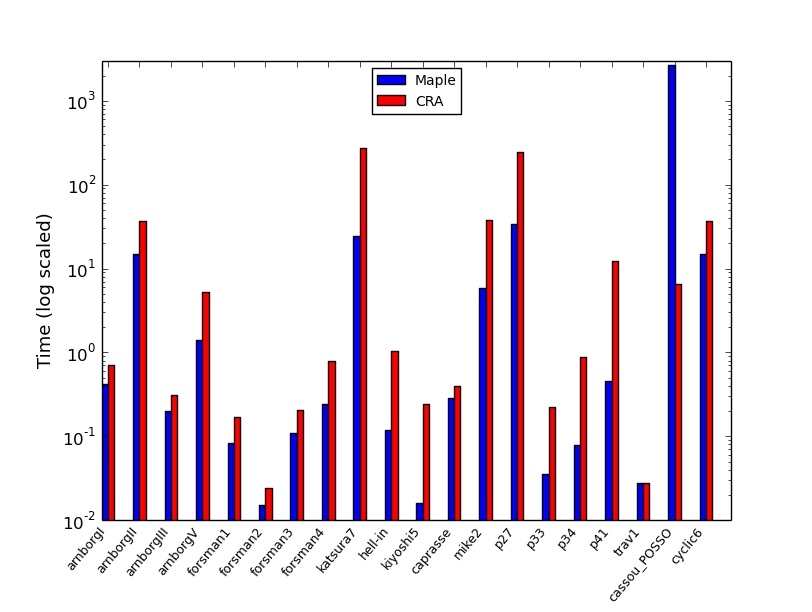
\includegraphics[scale=0.7]{bb_mapleVsCRA_modBasisTime.png}
  \caption{Buchberger's algorithm, comparing nonmodular to CRA mod basis time \label{fig:f4_tests}}
\end{figure}

\begin{figure}[H]
  \centering
  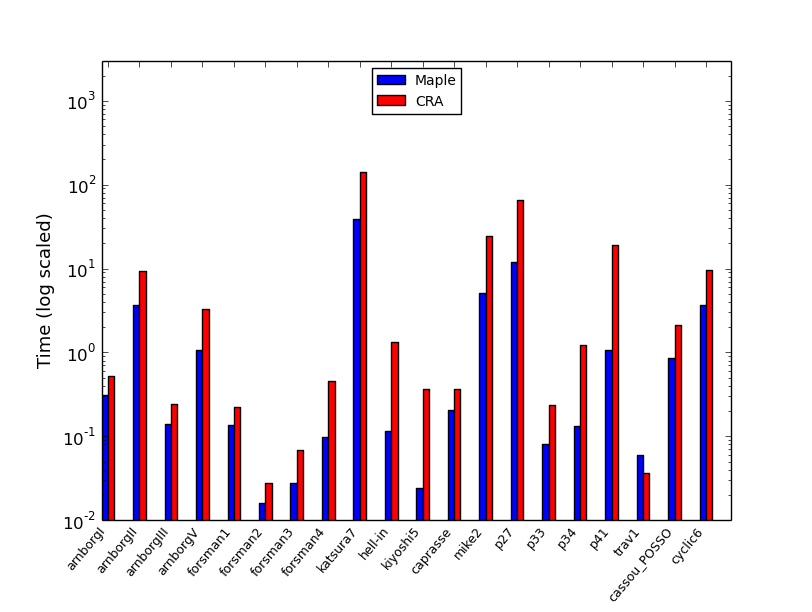
\includegraphics[scale=0.7]{f4_mapleVsCRA_modBasisTime.png}
  \caption{MapleF4 algorithm, comparing nonmodular to CRA mod basis time \label{fig:f4_tests}}
\end{figure}

\begin{figure}[H]
  \centering
  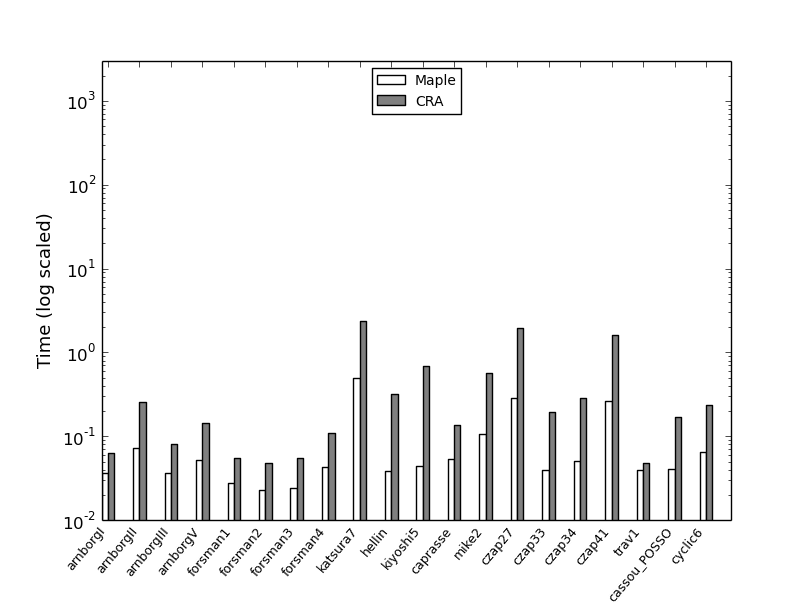
\includegraphics[scale=0.7]{fgb_mapleVsCRA_modBasisTime.png}
  \caption{FGB algorithm, comparing nonmodular to CRA mod basis time \label{fig:f4_tests}}
\end{figure}  

The above plots show that even with the modular basis computation time alone, the CRA basis method is already slower than the nonmodular basis computation.  Therefore, any added efficiency in terms of the Farey and CRA reconstruction methods using C or another optimization method would effectively be irrelevant, as the method cannot be any faster than the modular basis time alone, and this cannot be changed by the user.  

One potential alteration to the method would be to use different-sized primes; 16-bit primes were also used, however this was found to be slower (data included in \textbf{Appendix} \ref{appendix:supplData}).  

Going the other way and using bigger primes could be another approach, however this is also flawed.  The 64-bit Maple has a word-size of 64 bits; using primes greater than 32-bit would mean that their product would no longer be word-size, and therefore the computations would be in principle less efficient.  In addition, increasing the prime size would increase the intermediate expression swell.  Consider that in the limit of the primes reaching the maximum size of the final basis coefficients, then this modular computation would be exactly equivalent to the nonmodular method, and both methods should be equal in necessary time.  Removing the efficiency of using word-size primes for the computations means that the modular computations will not be faster than the nonmodular methods; at fastest, they would be equal to the nonmodular methods.  

So in conclusion, it seems that the current Maple Groebner package makes the attempted modular homomorphism methods redundant.  No added efficiency was observed; in fact, the modular approach was consistently slower than the basic nonmodular approach, for all available algorithms.  

However, this does not mean that the modular approach to Groebner basis computation is a dead end. 

\section{Future Research}    

Although in this case (considering Maple and the current Groebner package) the modular homomorphism approach turned out to decrease the time efficiency of the basis computations, there are various avenues to potentially explore in future research.  

In terms of Maple, the main roadblock is the inefficiency of the current modular basis computations.  Potentially, if a new release of Maple were to include a more efficient algorithm for the modular basis computation, this could tip the scales in favour of the modular approach.  Considering improvements to the existing Maple code, if the FGB code could include the capability of working over 32-bit primes this would increase the efficiency of the modular methods building the images using this algorithm.  The 32-bit primes were seen to be more efficient than the 16-bit primes for the other 2 algorithms, so it seems a logical conclusion that 32-bit prime processing would be faster in FGB as well.  

There are also computer algebra systems other than Maple.  Mathematica, Singular, and Python's sympy package all have Groebner plugins available; the experiment could be repeated using other available software packages.  

In particular, the sympy groebnertools package has the advantage of being open-sourced, and all the source code is readily available for user modification.  This package has implemented 2 algorithms for computing Groebner bases from a provided generating set and specified ordering: they have a modified Buchberger algorithm and Faugere's F5 algorithm.  Unlike the Maple package where the FGB C code is not provided for potential modification, sympy allows the user more freedom to add specialized functionality to the existing code base.  In this case, the modular homomorphism methods could be implemented into the groebnertools package itself, and the same experiment repeated.  External C plugins in Python could also be explored.

An efficiency test across platforms could also be made, to compare the efficiency of the various languages' implementations with respect to the problem set above.

%http://docs.sympy.org/0.7.6/_modules/sympy/polys/groebnertools.html 

\section{In Summary}

Although it removed the intermediate expression swell, computing the Groebner bases over modular integers, followed by modular reconstructions, did not increase the efficiency of the computation when implemented in the Maple system.  For the Hensel algorithm, this is due to the restriction of modular basis computation to the less efficient Buchberger algorithm, as it provides the required intermediate matrix.  The CRA, although more efficient than Hensel, is still slower than the Maple direct computation, as the modular basis computation time is greater than the time required for the single direct computation over the rationals.  The advancements in the Groebner basis computation methods make the homomorphic approaches effectively redundant in Maple.  However, one potential improvement to these algorithms could be the implementation of the modular methods in the fast FGB method implemented in C.  Additionally, other computer algebra systems could be tested through similar methods. 

\begin{appendices}

\chapter{Supplementary Definitions}\label{appendix:definitions}

This contains definitions which are presumed known and not explicitly declared in the text, but are referred to in passing.  They are included here for clarity.

\begin{defn}\label{defn: Unit}
  An element ${u \in D, \, D}$ domain, is a \textbf{unit} (\textbf{invertible}) if ${u}$ has a multiplicative inverse (i.e. with respect to operation ${*\,}$in ${D}$).

  For example, in $\mathbb{Z}$, the units are 1 and -1.
\end{defn}

\begin{defn}\label{defn: Associate}
  Two elements ${a, b \in D, \, D}$ domain, are \textbf{associates} if ${a \mid b}$ and ${b \mid a}$ i.e. they are multiples they are related via multiplication of a unit. 
\end{defn}

\begin{defn}\label{defn: Prime}
  An element ${p \in D - \{0\}, \, D}$ domain, is a \textbf{prime} if
  \begin{itemize}
    \item ${p}$ is \textbf{not} a unit
    \item whenever ${p = a \cdot b}$, for ${a, b \in D}$, then either ${a}$ or ${b}$ is a unit (but not both, since ${p}$ is not a unit)
  \end{itemize}
\end{defn}


\chapter{Implementation Details}\label{appendix:running}

\section{Batch Running}

This section gives a brief description of how the problems were timed.

The examples are included each in their individual Maple files; there is another Maple file which reads them all in and stores their initial ideal basis, problem name, and monomial ordering in parallel arrays.  The initial approach was to have one Maple file, \texttt{timer.mpl}, which ran each method and algorithm on each of the problems sequentially, printing the output of each to a named file before proceeding to the next problem.  This simple, Maple-only approach looping through all the problems was the naive approach, however it ran into issues with Maple's garbage collection: by the time the second problem was being computed, the memory from the first problem had not yet been released and was still taking up space in the Maple VM.  This caused two issues.
\begin{itemize}
  \item If the order of problem computations was reversed (i.e. if problems ran in order A then B, and then B then A), then the timings were significantly different; the second problem to execute always took much more time than if the same problem was executed first.  This is due to the additional memory which is taken up by the time the second problem begins executing; all the memory from the first is still taken up, and the extra garbage collections necessary to make room for the second computation adds additional time to the run.
  \item Another problem is the garbage collector itself; it seems to not deallocate memory even when the variable associated is reassigned or removed.  This leads to issues when multiple problems are computed sequentially in the same Maple session.  The Maple VM has a limited amount of memory on the server, and, even if this memory limit is increased, it is still a finite value.  The Groebner basis problems use so much memory that this limit is quickly reached, particularly when some of the Maple memory is already taken up from the previous problem.  When the memory limit is reached, the Maple session crashes with an error; this means that, if all the problems were computed in the same session, then the later problems would never be reached for computation as the kernel would run out of memory first.  
\end{itemize} 
The solution was to have one \texttt{timer.mpl} which computes one particular, specified problem, and a bash script to loop over all the problems and specify to the timer file which problem to run, and which combination of algorithm and method to use.

\begin{note}
  Maple does not provide the functionality of command line arguments as most programming languages provide.  For example, one cannot execute a Maple program by calling \begin{equation*}\texttt{maple mapleProgram arg1 arg2 ...}\end{equation*} specifying \texttt{arg1 arg2 ...} as command line arguments to the program.

  To get around this, the bash sed utility was used to modify the flag variables to specify which problem, algorithm, and method to run the timer with.
\end{note}

Then, all the problems are executed in their own Maple sessions to avoid any memory inconsistencies.

\section{Maple External C}


\chapter{Supplementary Data}\label{appendix:supplData}

The CRA was run using Buchberger and MapleF4 with 16-bit primes in addition to the 32-bit prime data included in the body of the thesis.  This was mainly done in order to have a more "level" comparison with the FGB CRA, which can only use 16-bit primes, as the option for larger primes has not been included in the CRA.  It was found that the 16-bit primes were slower than the 32-bit primes for Buchberger and F4; this seems to be due to the larger number of modular images which are necessary for the smaller primes, and that the majority of the time spent on CRA Groebner computations is in the calls to the modular basis computations in the Groebner package.

The FGB 16-bit prime data is included above in the \textbf{Methodology and Results} chapter.  

Note that, as above, the \textbf{DNF} problems are not included in the CRA data tables.

\singlespacing
\refstepcounter{Table}
\begin{center}
  \begin{tabular}{| l || r | r | r || r || r ||}
  \multicolumn{6}{l}{\textbf{Table \theTable}: CRA profiling, Buchberger algorithm (16-bit primes)}\TBstrut\\
  \hline 
  Problems & Mod Basis (s) & Farey (s) & CRA (s) & \textbf{Total} (s) & Images \\
  % Parameter & Average Relative Error & Variance of the Error \TBstrut \\ 
  \hline\hline
  arnborg1 & 1.093 & 0.023 & 0 & 1.116 & 4\\
  arnborg2 & 49.568 & 0.272 & 0.024 & 49.864 & 7\\
  arnborg3 & 0.582 & 0.024 & 0.007 & 0.613 & 4\\
  arnborg5 & 6.868 & 0.188 & 0.012 & 7.068 & 6\\
  forsman1 & 0.144 & 0.008 & 0 & 0.152 & 2\\
  forsman2 & 0.041 & 0.004 & 0 & 0.045 & 4\\
  forsman3 & 0.332 & 0.016 & 0 & 0.348 & 4\\
  forsman4 & 0.981 & 0.016 & 0.008 & 1.005 & 8\\
  katsura7 & 399.268 & 14.618 & 0.442 & 414.328 & 23\\
  hellin & 1.467 & 1.464 & 0.04 & 2.971 & 38\\
  kiyoshi5 & 0.534 & 1.461 & 0.041 & 2.036 & 135\\
  caprasse & 0.78 & 0.044 & 0 & 0.824 & 4\\
  mike2 & 54.882 & 1.807 & 0.1 & 56.789 & 13\\
  czap27 & 377.798 & 2.331 & 0.117 & 380.246 & 12\\
  czap33 & 0.302 & 0.297 & 0.017 & 0.616 & 31\\
  czap34 & 1.426 & 1.453 & 0.045 & 2.924 & 38\\
  czap41 & 20.023 & 14.799 & 0.553 & 35.375 & 77\\
  trav1 & 0.032 & 0 & 0 & 0.032 & 2\\
  cassou\_POSSO & 9.836 & 0.06 & 0.004 & 9.9 & 19\\
  cyclic6 & 50.378 & 0.279 & 0.031 & 50.688 & 7
  \\ % [1ex]
  \hline
  \end{tabular}
\end{center}

\refstepcounter{Table}
\begin{center}
  \begin{tabular}{| l || r | r | r || r || r ||}
  \multicolumn{6}{l}{\textbf{Table \theTable}: CRA profiling, MapleF4 algorithm (16-bit primes)}\TBstrut\\
  \hline 
  Problems & Mod Basis (s) & Farey (s) & CRA (s) & \textbf{Total} (s) & Images \\
  % Parameter & Average Relative Error & Variance of the Error \TBstrut \\ 
  \hline\hline
  arnborg1 & 0.816 & 0.036 & 0 & 0.852 & 4\\
  arnborg2 & 11.825 & 0.274 & 0.012 & 12.111 & 7\\
  arnborg3 & 0.437 & 0.028 & 0 & 0.465 & 4\\
  arnborg5 & 4.2 & 0.168 & 0.013 & 4.381 & 6\\
  forsman1 & 0.222 & 0.013 & 0 & 0.235 & 2\\
  forsman2 & 0.043 & 0.012 & 0 & 0.055 & 4\\
  forsman3 & 0.107 & 0.009 & 0 & 0.116 & 4\\
  forsman4 & 0.644 & 0.012 & 0 & 0.656 & 8\\
  katsura7 & 182.875 & 13.931 & 0.662 & 197.468 & 23\\
  hellin & 2.08 & 1.517 & 0.044 & 3.641 & 38\\
  kiyoshi5 & 0.677 & 1.487 & 0.036 & 2.2 & 135\\
  caprasse & 0.684 & 0.037 & 0 & 0.721 & 4\\
  mike2 & 29.621 & 1.707 & 0.247 & 31.575 & 13\\
  czap27 & 93.244 & 3.572 & 0.127 & 96.943 & 12\\
  czap33 & 0.371 & 0.265 & 0.004 & 0.64 & 31\\
  czap34 & 2.093 & 1.536 & 0.048 & 3.677 & 38\\
  czap41 & 31.701 & 15.124 & 0.456 & 47.281 & 77\\
  trav1 & 0.036 & 0.004 & 0 & 0.04 & 2\\
  cassou\_POSSO & 3.381 & 0.08 & 0.016 & 3.477 & 19\\
  cyclic6 & 11.676 & 0.283 & 0.021 & 11.98 & 7
  \\ % [1ex]
  \hline
  \end{tabular}
\end{center}
\doublespacing

Referring back to the 32-bit data tables for the CRA with these algorithms respectively, it is noted that the number of modular images here is the same as those necessary for the 16-bit FGB CRA, and close to twice that of the 32-bit CRA.  This is expected, as less prime images are necessary as the size of the prime increases; less primes are required for the product to be larger enough for the reconstruction to stabilize at the unique solution.

\end{appendices}






%----------------------------------------------------------------------
% END MATERIAL
%----------------------------------------------------------------------

% B I B L I O G R A P H Y
% -----------------------

% The following statement selects the style to use for references.  It controls the sort order of the entries in the bibliography and also the formatting for the in-text labels.
\bibliographystyle{plain}
% This specifies the location of the file containing the bibliographic information.  
% It assumes you're using BibTeX (if not, why not?).
\cleardoublepage % This is needed if the book class is used, to place the anchor in the correct page,
                 % because the bibliography will start on its own page.
                 % Use \clearpage instead if the document class uses the "oneside" argument
\phantomsection  % With hyperref package, enables hyperlinking from the table of contents to bibliography             
% The following statement causes the title "References" to be used for the bibliography section:
\renewcommand*{\bibname}{References}

% Add the References to the Table of Contents
\addcontentsline{toc}{chapter}{\textbf{References}}

\bibliography{uw-ethesis}
% Tip 5: You can create multiple .bib files to organize your references. 
% Just list them all in the \bibliogaphy command, separated by commas (no spaces).

% The following statement causes the specified references to be added to the bibliography% even if they were not 
% cited in the text. The asterisk is a wildcard that causes all entries in the bibliographic database to be included (optional).
\nocite{*}

\end{document}